\documentclass[12pt]{article}
\usepackage[margin=1in]{geometry}
%\usepackage{hyperref}
\usepackage{amsmath}
\usepackage{amsfonts}
\usepackage{graphicx}% http://ctan.org/pkg/graphicx
\usepackage{systeme}
%% tables
\usepackage{booktabs}
\usepackage{lscape}
\usepackage[table,xcdraw]{xcolor}
\usepackage{float}
\usepackage{url}

%% Make red text
\newcommand{\com}[1]{\textcolor{red}{ #1}}

%\linespread{2}

\usepackage[authoryear]{natbib}


\usepackage{tikz}
\tikzset{
  int/.style={circle, draw, fill=blue!20, minimum size=3em},
  init/.style={pin distance=1.2cm,pin edge={loop,thin,black}}
}
\usetikzlibrary{arrows,automata}

\pagenumbering{arabic}

\newcommand{\XX}{\ensuremath{25}} % number of methods

\newcommand{\xxsir}{\ensuremath{9} } % number of SIR methods
\newcommand{\wxxsir}{nine } % lower case number as word
\newcommand{\Wxxsir}{Nine } % capitalized word

\newcommand{\rr}{\ensuremath{\mathcal{R}_0}}

\setlength{\itemsep}{0pt}






\begin{document}

%%% draw a tree
\tikzset{
  treenode/.style = {shape=rectangle, rounded corners,
                     draw, align=center,
                     top color=white, bottom color=blue!20},
  root/.style     = {treenode, font=\Large, bottom color=red!30},
  env/.style      = {treenode, font=\ttfamily\normalsize},
  dummy/.style    = {circle,draw}
}




\title{\Wxxsir methods to estimate $\rr$ in the SIR model}
\author{ Shannon Gallagher$^{\dag}$, Andersen Chang$^{\ddag}$, and William F. Eddy$^{\dag}$ \\$\dag$ Department of Statistics and Data Science, Carnegie Mellon University\\ $\ddag$ Department of Statistics, Rice University}
\date{\today}
\maketitle

\begin{abstract}
For nearly a century, the initial reproduction number ($\rr$) has been used to summarize infectious diseases and to compare them to one another.  It is difficult to estimate $\rr$ due to assumptions on both how a disease transmits through a population and also due to differences in statistical estimation methods.  We describe nine methods used to estimate $\rr$ and provide a thorough simulation study of how these methods differ in the presence of disease parameters.  As real world motivation, we analyze the 2009 outbreak of the H1N1 pandemic influenza in the USA and compare the results from our nine methods to a previous study.  We discuss the most important aspects from our results which effect the estimation of $\rr$ and provide guidelines for estimating point estimates and confidence/credible intervals to create reliable, comparable estimates of $\rr$.
  \end{abstract}


\section{Introduction}\label{sec:intro}
What has been called ``arguably the most important quantity in the study of epidemics'' \citep{Heesterbeek2002},  $\mathcal{R}_0$, the initial reproduction number (by convention pronounced ``R-naught'') is an elusive quantity for epidemic modelers to estimate.  As defined by \citet{anderson1992}, $\rr$ is the ``the average number of secondary infections produced when one infected individual is introduced into a host population where everyone is susceptible.''  In some ways, $\rr$ summarizes an entire outbreak of a disease; it is used to assess whether a disease outbreak will occur and its severity.  Additionally, it describes what percentage of the population needs to be vaccinated to avoid such an epidemic, roughly $1-\rr^{-1}$, tells us the final size of the total number of infected individuals, and describes the probability of which we will observe an outbreak under the same conditions \citep{anderson1992,britton2010}).  Despite a clear definition of $\rr$, epidemiologists have struggled to create a standard  estimator for $\rr$  \citep{hethcote2000}.  A major issue in estimating $\rr$ is that the quantity is a \textit{property of the model}, meaning that $\rr$ is dependent not only on the usual noise that comes with statistical modeling but also on a variety of assumptions on how researchers assume a disease is transmitted through a population \citep{diekmann2009}.

To elaborate on $\rr$ being a property of the model, we first need to introduce the concept of the ``SI-framework,'' which was pioneered by Kermack and McKendrick in the 1920s \citep{getz2006}.   Here, S and I are known as compartments where S stands for ``susceptible'' and I for ``infectious.'' Infectious disease models then specify how individuals move from the S compartment to the I compartment.  Often, ancillary compartments are added such as R, which stands for recovered or dead, or E, which stands for exposed but not yet infectious.  The estimate of $\rr$ from a SIR model will not be directly comparable to the estimate of $\rr$ from a SEIR model, for example.  The difficulties of estimating $\rr$ are summarized and expanded upon by \cite{li2011}.  \cite{driessche2017} overviews a number of methods used to estimate $\rr$ but looks at systems beyond the SIR model and so these methods may not be directly compared.   As a result of $\rr$ being a property of the model, we limit our review to methods for estimating $\rr$ for the SIR model introduced by \cite{Kermack700}.

Even when limiting $\rr$ estimates to those from SIR models, estimation is still difficult.  Problems include mathematical versus statistical methods (i.e. solving for $\rr$ versus estimating $\rr$), the number of observations used to estimate $\rr$ (i.e. time), boundary cases of infection and recovery rates, population size, initial SI ratio, and restrictive assumptions placed upon the noise.  These are all issues for producing point estimates, to say nothing of issues related to confidence or credible intervals (CI).

We review \wxxsir methods for estimating $\rr$.  We note that these methods are not exhaustive but are chosen due to their impact and use in epidemiology.  We find that these methods also help to highlight the problems discussed above.

In addition to making a point estimate of $\rr$, we are particularly interested in the hypothesis  $H_0: \rr < \rr^*$, where $\rr^*$ may be the estimated reproduction number of a past outbreak of the same disease, an outbreak of a different disease in the same region, or a value of 1.  An estimate of $\hat{\rr}<1$ indicates that the disease will die out.  We do note that the last situation is situational as we generally only observe diseases that do outbreak and inherently have a value greater than 1.  However, \cite{britton2010} provides guidance on the probability of observing an outbreak based on $\rr$ (that is estimated final size is approximately the probability of us observing an outbreak)   We also discuss techniques for estimating CIs for each of the different methods.  These CI estimates are created using the delta method, the block bootstrap, and the posterior distribution \citep{cao1999,wasserman2004}.

In the following sections, we present a series of simulations in which we examine each of our $\rr$ estimation methods.  Within these simulations, we vary the number of observations used to estimate $\rr$, infection and recovery rates, the total population size, initial SI ratio, and several assumptions about the noise.  After analyzing our simulations, we apply our methods to data from the USA H1N1 influenza pandemic.


Finally, we discuss our recommendations for estimating $\rr$ in the SIR model, and we comment on how these recommendations extend to more complex epidemiological models beyond the SIR model and on how many of the problems with estimating $\rr$  become exacerbated in such models.


The rest of this manuscript is organized as follows.  In Section \ref{sec:r0}, we briefly discuss the origin of $\rr$.  In Section \ref{sec:sir-intro}, we introduce the SIR model as described by \cite{Kermack700}.  In Section \ref{sec:methods}, we overview the \wxxsir methods for estimating $\rr$. In Section \ref{sec:ci}, we discuss how to estimate CIs for each of the \wxxsir methods.  In Sections \ref{sec:sim-res} - \ref{sec:sim-var-res}, we present the results of our simulations.  In Section \ref{sec:real-data}, we evaluate the methods on real data--from the USA H1N1 influenza pandemic of 2009.  Finally, in Section \ref{sec:discussion}, we provide recommendations of estimating $\rr$ for the SIR model and offer comments on how these conclusions extend to more complex models.


\subsection{Origins and Difficulties of Estimating $\rr$}
\label{sec:r0}

The origins of $\rr$ are tied to the survival function, which originates from the field of demography in the late 1800s.  The survival function describes how many female offspring a woman is expected to produce in her lifetime, literally the reproduction number \citep{dietz1993estimation}.  In demography, we have
\begin{align}\label{eq:surv}
\rr = \int_0^\infty p(a) \beta(a) da
\end{align}
where $p(a)$ denotes the probability of a woman surviving to age $a$ and $\beta(a)$ the rate of an individual of age $a$ giving birth to a  girl.  The concept of the reproduction number was later imported to the field of epidemiology by MacDonald and Smith \citep{dietz1993estimation}.  Analogously in epidemiology, $p(a)$ is the age of a disease, and $\beta(a)$ is the infection rate at time $a$.

Equation \ref{eq:surv} is the chronologically first, and in many ways, the most direct method to estimate $\rr$.  The premise of this whole paper is based upon the fact that estimating $\rr$ from the survival function in Equation \eqref{eq:surv} is a difficult task.  It is due to this difficulty that other estimates even exist and why we must treat $\rr$ as a property of the SIR model.

Other difficulties in estimating $\rr$ arise from model assumptions on how randomness enters the model and sensitivity of the estimate to changes in the model parameters.  For example, the SIR model is special in that two of its compartments, S and R are monotonic.  The number of susceptibles is non-increasing and the number of susceptibles is non-decreasing.  Logically, models should enforce this monotonicity of the two compartments.  As a consequence, this restricts assumptions on how randomness enters the model.  For example, Gaussian error, a common assumption in statistics and machine learning, becomes highly suspect due to the non-symmetrical nature of the noise imposed by the monotonic $S$ and $R$ compartments. 

These difficulties in estimating $\rr$ have led a number of researchers to analyze the sensitivity of $\rr$ with respect to small perturbations in parameters like $\beta$ and $\gamma$, respectively the infection and recovery rate \citep{lash2003,epstein2007agent,capaldi2012}.  Even this is a difficult task. Since there is no analytic solution to the SIR model, estimating the set of derivatives with respect to $\beta$ and $\gamma$ must be done numerically, which can substantially increase computation time.  We should note that this sensitivity analysis is done before even adding any distributional assumptions on how randomness enters the model.

Below in Table \ref{tab:r0-real-ex}, we provide examples of estimates of $\rr$ for specific diseases from publications over the past three decades, spanning various locations over the world.  We display estimates for HIV, Zika (ZIK-V), Ebola (EVD), seasonal influenza, pandemic H1N1 influenza A, and measles.  These estimates of $\rr$ are not limited to those of the SIR model, although many of the displayed results originate from this framework.  Of these, measles seems to have the largest estimated values of $\rr$, followed by Zika, Ebola, H1N1 influenza, seasonal influenza, and HIV.  We see that African locations seem to have larger estimates of $\rr$ compared to the rest of the world, regardless of the disease.  Some of the accompanying intervals (not necessarily CIs) are extremely large such as the case of HIV in Uganda (Interval: [0.12, 14.17]) whereas some are extremely small such as for Ebola in Guinea (Interval: [1.50, 1.52]).  We see that estimates for H1N1 influenza are generally higher than that of seasonal influenza, although we find that in our appliaction the opposite is true.  The lowest possible estimate for $\rr$ reported is 0.12 for HIV in Uganda, and the largest is 17.00 for measles in England and Wales.  Within diseases, we see that estimates for $\rr$ seem to be similar, although typically do not lie in one another's intervals, suggesting that there is disparity in estimates of $\rr$.

% Please add the following required packages to your document preamble:
% \usepackage{booktabs}
% \usepackage{graphicx}
% \usepackage{lscape}
\begin{landscape}
\begin{table}
\centering
\begin{tabular}{@{}lllrrrl@{}}
\toprule
\textbf{Disease}    & \textbf{Location}                & \textbf{Year(s)}                 & \textbf{$\rr$} & \textbf{Lower} & \textbf{Upper} & \textbf{Source}                                                                                                                  \\ \midrule
HIV                 & Belgium                          & 2004-2010                     & 1.10          & 1.09           & 1.16           & \cite{coelho2011}   \\
HIV                 & Netherlands                      & 2004-2010                     & 1.11        & 1.10            & 1.18           & \cite{coelho2011}    \\
HIV                 & Portugal                         & 2004-2010                     & 1.08        & 1.06           & 1.15           & \cite{coelho2011}   \\
HIV                 & San Francisco, USA               & 1993                          & 5.00           & 2.00              & 8.00              & \cite{blower1994}    \\
  HIV                 & Uganda                           & 2002-2008                     & 3.31        & 0.12           & 14.17          & \cite{nsubuga2014}    \\ \hline
ZIK-V                & Colombia - Barrranquilla           & 2015                          & 2.40         & 3.80            & 5.60            & \cite{towers2016}    \\  
  ZIK-V                & Colombia                         & 2015-2016                     & 2.50         & 3.00              & 3.60            & \cite{nishiura2016}    \\
ZIK-V                & Colombia                         & 2015                          & 1.42        & 2.56           & 3.83           & \cite{majumder2016}  \\
ZIK-V                & French Polynesia                 & 2013                          & 2.75        & 2.53           & 2.98           & \cite{zhang2017}        \\
ZIK-V                & French Polynesia                 & 2013-2014                     & 3.70         & 2.60            & 4.80            & \cite{kucharski2016}  \\
  ZIK-V                & Florida                          & 2016                          & 0.16        & 0.13           & 0.19           & \cite{dinh2016}       \\ \hline
EVD                 & Democratic Republic of the Congo & 1995                          & 2.70         & 1.90            & 2.80            & \cite{legrand2007}  \\  
  EVD                 & Guinea                           & 2014                          & 1.51        & 1.50            & 1.52           & \cite{althaus2014}   \\
  EVD                 & Liberia                          & 2014                          & 1.59        & 1.57           & 1.60            & \cite{althaus2014}    \\
  EVD                 & Sierra Leone                     & 2014                          & 2.53        & 2.41           & 2.67           & \cite{althaus2014}      \\
EVD                 & Uganda                           & 2000                          & 2.70         & 2.50            & 4.10            & \cite{legrand2007}   \\
EVD               & Western Africa                   & 2014                          & 1.78        & 1.60            & 2.00              & \cite{fisman2014}   \\
EVD & Western Africa                   & 2014                          & 1.60         & 1.40            & 1.80            & \cite{towers2014}  \\
\hline
Seasonal Influenza  & Australia, France, USA          & 1972-2002 & 1.30         & 1.20            & 1.40            & \cite{chowell2008}  \\
  Seasonal Influenza  & French Territory                 & 1987-1995                     & 1.50         & 1.09           & 1.73           & \cite{bonabeau1998}  \\ \hline
  H1N1 Influenza     & Peru                             & 2009                          & 1.37        & 1.20            & 1.70            & \cite{desilva2009}        \\   
H1N1 Influenza      & Thailand                         & 2009                          & 2.07        & 1.92           & 2.22           & \cite{desilva2009}     \\
  H1N1 Influenza & USA & 2009 & 1.50 & 1.30 & 1.70 &\cite{towers2009} \\ \hline
  Measles     & Canada - Ontario                  & 1912-1913                         & 11.50        & 11.00           & 12.00            & \cite{anderson1992}     \\
    Measles     & Eastern Nigeria                  & 1960-1968                          & 16.50        & 16.00          & 17.00           & \cite{anderson1992}     \\
  Measles      & England - Cirencester                 & 1947-1950                          & 13.50   & 13.00           & 14.00            & \cite{fraser2009}     \\
  Measles     & England - Willesden                  & 1912-1913                          & 11.00        & 12.00       & 1.60            & \cite{anderson1992}     \\  
  Measles     & England and Wales                  & 1950-1968                          & 17.00      & 16.00          & 18.00         & \cite{anderson1992}     \\
    Measles     & Ghana                 & 1960-1968                          & 14.50       & 14.00          & 15.00            & \cite{anderson1992}     \\
  Measles     & USA - Kansas                  & 1918-1921                          & 5.50    & 5.00          & 6.00          & \cite{anderson1992}     \\
\bottomrule
\end{tabular}
\caption{Estimates of $\rr$ from various researchers for the infectious diseases of HIV, (Zika) ZIK-V, Ebola (EVD), seasonal influenza, and H1N1 pandemic influenza ranging from the years 1972-2016 in various locations.  We also report the lower and upper bounds reported by the researchers.}
\label{tab:r0-real-ex}
\end{table}
\end{landscape}



\subsection{Kermack and McKendrick's SIR Model}
\label{sec:sir-intro}

The SIR model introduced by \cite{Kermack700} is a compartment model, where individuals move from susceptible, to infectious, and finally recovered states.  We make five essential assumptions,
\begin{enumerate}
\item The compartments are discrete and have no overlap.
\item The transition of objects into and out of compartments is described by a set of known equations, possibly dependent on unknown parameters.
\item The populations mix homogeneously.
\item The number of objects in each compartment at time $t=0$ is known.
  \item The law of mass action is followed.
  \end{enumerate}  


The law of mass action is a property borrowed from chemistry which says that the mass of the product per unit time is proportional to the mass of the reactants \citep{lotka1920}.  In epidemiology, this means that the proportion of new infections per unit time is proportional to the current  number of susceptible \citep{anderson1992}.  
 

In this particular  SIR model (displayed in Figure \ref{fig::sir}), the number of individuals ($N$) is constant. Adaptations of the SIR model can include birth and death rates, which may correspondingly change the derivation of $\rr$ (for further discussion, see Section \ref{sec:discussion}). The parameters  $\beta$ and $\gamma$ have epidemiological meaning.  Here, $\beta$ is the average infection rate and $\gamma$ is the average recovery rate.  The movement of individuals from one compartment to another is represented through the ordinary differential equations below.  Both $\beta$ and $\gamma$ are constrained to be between $0$ and $1$.  For the remainder of this paper, we use $X$, $Y$, and $Z$ to denote the number of individuals in the $S$, $I$, and $R$ compartments, respectively, to avoid any confusion with $\rr$.
\begin{align}
\systeme{\frac{dX}{dt} = -\frac{\beta XY}{N}, \frac{dY}{dt} = \frac{\beta XY}{N} - \gamma Y, \frac{dZ}{dt} = \gamma Y}. \label{eq:sir}
\end{align}
In words, susceptible individuals become infected at a rate that is proportional to the percentage of infected individuals multiplied by $\beta$, the infection rate, and the number of susceptible individuals.  Infectious individuals recover at a rate of $\gamma$ multiplied by the number of infected individuals.




The SIR model is represented graphically in Figure \ref{fig::sir}. 
\begin{figure}[h]
\centering
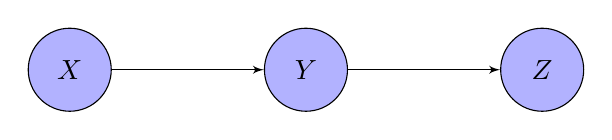
\begin{tikzpicture}[node distance=3cm,auto,>=latex',every node/.append style={align=center}]
    \node [int,  fill = white!70!blue] (a)              {$X$};
    \node [int,  fill = white!70!blue]           (c) [right of=a] {$Y$};
    \node [int,  fill = white!70!blue] (e) [right of=c] {$Z$};
    \path[->, auto=false] (a) edge node {} (c)
                          (c) edge node {} (e) ;
\end{tikzpicture}
\caption{Depiction of a SIR model where $X=S, Y=I,$ and $Z=R$.  One can only be infected once by the disease once in this model.}\label{fig::sir}
\end{figure}
Since the number of indivudals ($N$) is constant, then
\begin{align*}
\frac{dX}{dt} + \frac{dY}{dt} + \frac{dZ}{dt} \equiv 0.
\end{align*}
An outbreak occurs if the rate of change of infectious individuals is positive, $\frac{dY}{dt} > 0$, or equivalently,
\begin{align*}
  \frac{dY}{dt} &> 0 \\
  \implies -\frac{dX}{dt} - \frac{dZ}{dt} &> 0 \\
  \implies \frac{\beta X Y}{N}  - \gamma Y &> 0 ,\\
\implies  Y \left ( \beta \frac{X}{N} - \gamma \right ) & > 0\\
\implies   \frac{\beta}{\gamma} &> \frac{N}{X}.
\end{align*}
That is,  the rate of new infections is greater than the rate of recovery.  So as long as the number of initially susceptible individuals is large compared to the total population, $\frac{X}{N} \approx 1$, then an outbreak will occur if $\rr >1$,
\begin{align*}
  \rr \overset{def}{=} \frac{\beta}{\gamma}.
  \end{align*}
  To incorporate randomness into the model, we add noise, namely,
  \begin{align}\label{eq:sir-noise}
    \hat{X}(t) &= X(t) + \epsilon_{X,t}\\
    \hat{Y}(t) &=  N - \hat{X}(t) -\hat{Y}(t)  \nonumber\\
    \hat{Z}(t) &= Z(t) - \epsilon_{Z,t}. \nonumber
  \end{align}
The ``hats'' in Equation \ref{eq:sir-noise} are used to distinguish real, observed data from the ``true'' model without hats.  We are assuming the observations are generated based on the  deterministic ODEs (possibly converted to discrete time) presented in Equation \ref{eq:sir} with time and compartment dependent noise $\epsilon_{X,t}$ and $\epsilon_{Z,t}$.  Since, $N$, the total population, is constant, then $\hat{Y}$ is adjusted accordingly.

In summary, when we discuss estimators for $\rr$ for the SIR model, we mean to say we are forming an estimator of $\rr$ from the given set of data in Eq. \ref{eq:sir-noise},
\begin{align*}
  \textnormal{Data} &= \left \{\left (\hat{X}(t), \hat{Y}(t), \hat{Z}(t) \right ) : t=0, 1, \dots, T\right \}, \\
  \hat{\rr} &= m(\textnormal{Data}),
\end{align*}
where $m$ is a function of the data.

Good properties of an estimator may include (1) being a consistent estimator
\begin{align*}
  \hat{\rr} \overset{P}{\to} \rr \textnormal{ as } T\to \infty,
\end{align*}
where `$\overset{P}{\to}$' stands for convergence in probability or (2) converging to a known probability distribution (convergence in distribution `$\overset{d}{\to}$' \citep{wasserman2004}),
\begin{align*}
\hat{\rr} \overset{d}{\to} F.  
\end{align*}
As we are interested in the hypothesis
\begin{align*}
  H_0:\;& \rr < \rr^* \\
  H_A:\;& \rr \ge \rr^*
\end{align*}
Then for some $\alpha \in [0,1]$, we would like to know for some $\hat{a}, \hat{b} >0$
\begin{align*}
P(\hat{a} \le \rr \le \hat{b}) \le 1 - \alpha.
\end{align*}
This property is particularly desirable, as we can estimate $\hat{a}$ and $\hat{b}$ from the distribution $F$.  At any rate, we would like to be able to estimate $\hat{a}$ and $\hat{b}$ for a given $\alpha$-level.  We could also make similar hypothesis tests such as  $\rr$ for H1N1 influenza is greater than the reported $\rr$ for seasonal influenza.

\subsection{$\rr$ is a property of the model}

We provide an example of how $\rr$ is a property of the model.  Consider the situation of data generated from an SEIR (XEYZ) model (described by \cite{cintronarias2009}), generated from the following ODEs,

\begin{align*}
  \frac{dX}{dt} &= - \frac{\beta_{XEYZ} XY}{N} \\
  \frac{dE}{dt} &= \frac{\beta_{XEYZ} XY}{N}  - \mu_{XEYZ} E\\
  \frac{dY}{dt} &= \mu_{XEYZ} E - \gamma_{XEYZ} Y \\
  \frac{dZ}{dt} &= \gamma_{XEYZ} Y,
\end{align*}
again, with a constant population of $N$ and with known initial values $(X(0), E(0), Y(0), Z(t))$.  The parameter $\mu_{XEYZ}$ is the rate at which latently exposed individuals become infectious.  The subscript ``XEYZ'' is used to emphasize that the disease parameters (especially $\beta$ and $\gamma$) are different than of those in the XYZ model.  The reproduction number for the XEYZ model, is $\rr = \frac{\beta_{XEYZ}}{\gamma_{XEYZ}}$, compared to the reproduction number for the XYZ model, $\rr = \frac{\beta_{XYZ}}{\gamma_{XYZ}}$.

Consider the case when $N=10000, (\beta, \gamma) = (.06, .03)$, $(X(0), E(0), Y(0), Z(t)) = (9500, 0, 500, 0)$ for times $t=1, \dots, 365$.  Let the parameter $\mu$ range between [0.005, 0.250].  This generates data set
$$D_{\mu, \textnormal{XEYZ}} = \left \{(\hat{X}_{XEYZ}(t), \hat{E}_{XEYZ}(t), \hat{Y}_{XEYZ}(t), \hat{Z}_{XEYZ}(t): t=1, \dots, 365\right \},$$
which is observed by researcher 1.  Now assume that researcher 2 misspecifies the model for this data as a SIR (XYZ) model rather than a SEIR (XEYZ) model.  That is, she observes all non-infectious individuals as susceptibles and generates data sets
$$D_{\mu, XYZ} = \left \{\hat{X}_{XYZ}(t) = X_{XEYZ} + E_{XEYZ}, \hat{Y}_{XYZ} = Y_{XEYZ}, \hat{Z}_{XEYZ} = Z_{XYZ} : t = 1, \dots, 365 \right \}.$$
This situation is illustrated in Figure \ref{fig:sir-vs-seir} with $\mu = 0.01$.

\begin{figure}
  \centering
  \includegraphics[width=.9\textwidth]{images/seir-sir-data.pdf}
  \caption{Top: XEYZ generated data over the course of a year.  Bottom: data tranformed from the XEYZ model to the XYZ model by combining all X and E compartments from the XEYZ model for the X compartment in the XYZ model.}\label{fig:sir-vs-seir}
  \end{figure}

Both researchers want to estimate $\rr$ and so fit models to their data sets.  The details of how the models are fit are not so important at the moment (but will be in the later sections), but to fairly compare one model to another assume both researchers use a least squares estimates to estimate the disease parameters and then use the ratio estimator (RE) as an estimate of $\rr$.  That is researcher 1 estimates $\rr$ with
\begin{align*}
  (\hat{\beta}_{XEYZ}, \hat{\gamma}_{XEYZ}, \hat{\mu}_{XEYZ} )&=\arg \min_{\beta, \gamma, \mu} \sum_{t} \left [ \left (X_{XEYZ}(t) - X(t)\right )^2  \right . \\
                                                                 &+\left ( E_{XEYZ}(t) - E(t) \right )^2  \\
  &\left . + \left ( Z_{XEYZ}(t) - Z(t) \right )^2\right ]
\end{align*}
Then the RE for $\rr^{XYZ}$ is given by Equation \ref{eq:sirls},
\begin{align*}
  \hat{\rr}^{XEYZ}= \frac{\hat{\beta}_{XEYZ}}{\hat{\gamma}_{XEYZ}}.
\end{align*}
Researcher 2 estimates $\rr$ with 
\begin{align*}
(\hat{\beta}_{XYZ}, \hat{\gamma}_{XYZ} )&=\arg \min_{\beta, \gamma} \sum_{t} \left [ \left (X_{XYZ}(t) - X(t)\right )^2 + \left ( Z_{XYZ}(t) - Z(t) \right )^2 \right ].
\end{align*}
Then the RE for $\rr^{XYZ}$ is given by Equation \ref{eq:sirls},
\begin{align*}
  \hat{\rr}^{XYZ}= \frac{\hat{\beta}_{XYZ}}{\hat{\gamma}_{XYZ}}.
\end{align*}

We plot the two estimates of $\rr$ as a function of $\mu$ in Figure \ref{fig:r0-alpha}.  We should note we also estimated the standard errors of the estimates of $\rr$, but they do not show up on the figure because they are of the order of $10^{-4}$.  Unsurprisingly, under the SEIR model speficiation, $\hat{\rr}=2$ because there is no noise in the data, and the data is generated from an SEIR model.  However, as we see in Figure \ref{fig:r0-alpha} the RE of $\hat{\rr}$ from the SIR model for small values of $\mu$ (a long latency period) can result in double the size of $\hat{\rr}$!

\begin{figure}
  \centering
  \includegraphics[width=\textwidth]{images/r0-est.pdf}
  \caption{Estimates of $\rr$ from both the XEYZ and XYZ model specification for different values of $\mu$.}\label{fig:r0-alpha}
  \end{figure}


For those readers not convinced by our small example, we offer this mathematical intuition of the next generation model (NGM).

 The NGM is a generalization of any compartment model at the infection-free steady state ($Y(t)=0$ and all derivatives with respect to time sum to zero). Originally, introduced by \citep{diekmann1990}, \cite{diekmann2009} posit a recipe to find $\rr$ for a wide class of compartment models, including SIR and SEIR. First, define the infected subsystem as ``the equations of the ODE system that describe the production of new infections and changes in state among infected individuals.''  Let $x = (C_1, C_2, \dots, C_m)^T$ where $C_i$ are the different compartments of the infected subsystem.  The steps to find $\rr$ are as follows:


\begin{enumerate}
\item Take the subsystem of infected individuals (including those who have been exposed) and linearize the subsystem about the infection-free steady state
\item Decompose the linearized infected subsystem into $(T + \Sigma )x$ where $T$ is a $m\times m$ matrix of \textit{transmissions} and $\Sigma$ is a $m \times m$ matrix of \textit{transitions}.
\item $\rr$ is the spectral radius (i.e. the dominant eigenvalue) of $-T \Sigma^{-1}$.  
\end{enumerate}

Here, $T_{ij}$ is the rate of transmission of \textit{newly} infected individuals in state $i$ created by individuals in state $j$.  $\Sigma_{ij}$ is the transition rate of individuals into compartment $i$ from compartment $j$.

This method has the assumptions of a basic compartment model: homogeneous mixing among populations and the law of mass action, i.e., that the number of infected individuals are proportional to the number of infected individuals at the previous step.   Additionally, this method is advantageous in that the matrix $-\Sigma^{-1}$ has intuitive meaning.  The $ij$th entry of $- \Sigma^{-1}$ is the ``expected time that an individual who presently has state $j$ will spend in infected state $i$.''

The NGM shows that $\rr$ is the spectral radius of a matrix which is composed of the transmission of disease to susceptible individuals and transition of individuals among the other compartments.  $\rr$ is thus a property of the model.

Following the examples presented in \cite{diekmann1990}, for the SIR (XYZ) model, the linearized infection-free sub-system occurs when $Y(t)=0$ and $X(t)=N$ and is
\begin{align*}
\frac{dY}{dt} &= - \beta_{XYZ} Y + \gamma_{XYZ} .
  \end{align*}
  Then $T= \beta_{XYZ}$ (the rate of new infections) and $\Sigma = -\gamma_{XYZ}$.  Then $K = \frac{\beta_{XYZ}}{\gamma_{XYZ}}$ which is also, trivially, the dominant eigenvalue, and hence, $R_0 = \frac{\beta_{XYZ}}{\gamma_{XYZ}}$.

We can also derive the NGM for the SEIR (XEYZ) model.  We have an infection-free steady state when $E=Y=0$ and set $X=N$.  Then $x = (E, Y)^T$ is the infected subsystem.  The linearized subsystem is
  \begin{align*}
  \left \{
  \begin{array}{cl}
    \frac{dE}{dt} &= \beta_{XEYZ} Y  - \mu_{XEYZ} E\vspace{.5em}\\
    \frac{dY}{dt} &=  \mu_{XEYZ} E  - \gamma_{XEYZ} Y \\
  \end{array}
  \right .
  \end{align*}
  Then $T = \left ( \begin{array}{cc} 0 & \beta_{XEYZ} \\ 0 & 0  \end{array} \right )$ and $\Sigma = \left ( \begin{array}{cc} -\mu_{XEYZ} & 0 \\ \mu_{XEYZ} & - \gamma_{XEYZ} \end{array} \right )$, and $K =\left ( \begin{array}{cc} 0& \beta_{XEYZ} / \gamma_{XEYZ} \\ 0 & 0 \end{array} \right  )$.

  Then the spectral radius of $K$ is $R_0  = \frac{\beta_{XEYZ}}{\gamma_{XEYZ}}$, which makes sense as exposed individuals are not contributing to the number of new infections.

  Although the $\rr$ ends up being similar (infection rate over the recovery rate) for both the SIR (XYZ) and SEIR (XEYZ) models, the derivations are different because of the addition of the exposed compartment.  In general, more complicated models will result in different derivations of $T$ and $\Sigma$ and hence different derivations of $\rr$.




\section{Overview of \wxxsir methods to estimate $\rr$ for the SIR model}
\label{sec:methods} 

In this section, we describe the \wxxsir methods in detail, including advantages and disadvantages of each.

\subsection{Ratio Estimator ($\beta$, $\gamma$) (RE)}\label{least-squares-beta-gamma}
Our first approach to estimate $\rr$ in the SIR model is to minimize the joint mean square error for the data collected at each time point and use the plug-in estimator found in Equation \ref{eq:sirls}.  In particular, we find

\begin{align*}
(\hat{\beta}, \hat{\gamma} )&=\arg \min_{\beta, \gamma} \sum_{t} \left [ \left (\hat{X}(t) - X(t)\right )^2 + \left ( \hat{Z}(t) - Z(t) \right )^2 \right ]
\end{align*}
Then the ratio estimator (RE) estimate for $\rr$ is given by Equation \ref{eq:sirls},
\begin{align}\label{eq:sirls}
  \hat{\rr}= \frac{\hat{\beta}}{\hat{\gamma}}.
\end{align}

The estimate resulting from this method are often found via a grid search of $\beta$ and $\gamma$ values to minimize the squared error.  The estimates can also be found using more sophisticated optimization algorithms. Since we typically cannot explicitly write down the partial derivatives of $S$, $I$, and $R$ with respect to $\beta$ and $\gamma$, we can only use minimization algorithms which do not rely on an explicit gradient such as Nelder-Mead simplex minimization \citep{nelder-mead1965}.

A reasonable question one may ask is why use the $L_2$-norm as opposed to $L_1$ or some other similarity score.  A possible answer is that if we were to assume Gaussian noise, then the $L_2$-norm would be equivalent to the maximum likelihood estimation.  Another answer is that $L_2$ is a continuously differentiable function and hence is easier to compute, which allows for sensitivity analysis to  be conducted more easily.  Finally, the RE estimate can be found without writing down explicit assumptions about the noise within the model.  However, we cannot guarantee properties of consistency or convergence to a known distribution without more explicit assumptions.  

On the other hand, the RE is easy to implement using software such as \texttt{R}'s \texttt{optim()} function, and as we see in Section \ref{sec:results} produces results comparable to other methods.  RE and similar variants have been used to estimate $\rr$ in \cite{majumder2016}.

\subsection{Reparametrized Ratio Estimator ($\rr$, $\gamma$) (rRE)}\label{reparametrized-least-squares-rux5f0-gamma}

In the previous method (Section \ref{least-squares-beta-gamma}), we estimated $\beta$ and $\gamma$ and then estimated $\rr$.  However, it is possible to directly estimate $\rr$ if we reparametrize the ODEs in Equation \eqref{eq:sir} directly with \(\rr\) and \(\gamma\), using the relation $\rr = \frac{\beta}{\gamma}$; this yields

\begin{align*}
  \left \{
  \begin{array}{cl}
    \frac{dX}{dt} &= - \rr \gamma Y \frac{X}{N}\vspace{.5em}\\
    \frac{dY}{dt} &=  \rr \gamma Y \frac{X}{N}  - \gamma Y\vspace{.5em} \\
    \frac{dZ}{dt} &=  - \gamma Y 
  \end{array}
  \right . .
  \end{align*}
We find
\begin{align*}
(\hat{\rr}, \hat{\gamma} ) &= \text{argmin}_{\rr, \gamma} \sum_{t} \left [ \left (X_{obs}(t) - X(t)\right )^2 + \left ( Z_{obs}(t) - Z(t) \right )^2 \right ]
\end{align*}
We use the $\hat{\rr}$ directly from the above estimation problem, which again can be found with a grid search or another optimization process.  It may be surprising that this method leads to different results than simply using the ratio estimator.  We also see that this method results in different standard errors than in RE, which we discuss further in Section \ref{sec:results}.

Like RE, while we have no explicit assumptions on the noise, we also are uncertain of any theoretical properties of our resulting estimator.  Likewise, the same difficulties in sensitivity analysis arise as for the RE.



\subsection{Linear Model Approximation (LMA)}\label{linear-model-approximation-degree-10}

The SIR ODEs in Eq. \ref{eq:sir} have no known closed form solution, and so we use numerical integration to obtain approximate solutions.  In addition to this, data collected from real diseases are typically very noisy to begin with.  The SIR model may be approximated by a linear model.  We use this method to estimate $\rr$.

Specifically, we estimate two polynomials in \(t\) with degree $K$  to \(X_{obs}\)
and \(Z_{obs}\) using least squares to find the coefficients $\{(\hat{x}_k,
\hat{z}_k)\}_{k=1, \dots, K}$,
\begin{align*}
\hat{X}(t) &= \sum_{k=0}^K \hat{x}_k t^k\\
{\hat{Z}}(t) &= \sum_{k=0}^K \hat{z}_k t^k
\end{align*}
Then, we estimate the derivatives as
\begin{align*}
\hat{X}^\prime(t) &= \sum_{k=1}^K k \hat{x}_k t^{k-1}\\
\hat{Z}^\prime(t) &= \sum_{k=0}^K k \hat{z}_k t^{k-1}
\end{align*}
Following,  an estimator for \(\rr\) is derived from the ODEs in Equation \eqref{eq:sir},
\begin{align}
  - \frac{X^\prime}{Z^\prime}&= \rr \frac{X}{N} \nonumber\\
  \rr &=       -\frac{X^\prime}{
        Z^\prime} \cdot \frac{N}{X} \nonumber\\
  \hat{\rr} &= -\frac{\hat{X}^\prime(0)}{ \hat{Z}^\prime(0)} \cdot \frac{N}{\hat{X}(0)}. \nonumber
  \end{align}
  Here, $K$ is arbitrary and should be selected using some criterion such as AIC.  Besides optionally deciding on the degree of polynomials to fit, this model is simple to implement and gives comparable results to using the ratio estimator with the SIR model.  The time $t=0$ is used to best capture the initial outbreak.

  An advantage of using this estimation method is that it is simple to implement using any linear modelling software.  On the other hand, we assume $X(t) = \hat{X}(t)$ and so if the data truly follows the SIR model, then we will likely have a result for $\rr$.  Using this method, we are able to check how sensitive $\rr$ is to the degree of the fitted polynomial.

\subsection{Linear Model Approximation, All Time Points (LMAT)}\label{linear-model-approximation-all-time-points-degree-10}

The above formulation (Section \ref{linear-model-approximation-degree-10}) of a linear model approximation only uses the estimate at time $t=0$ to estimate $\rr$.  We can instead, use all time points $T$ available to estimate $\rr$.  We fit a polynomial in \(t\) with degree \(K\) to \(X_{obs}\)
and \(Z_{obs}\) as above, with a slight modification in how we estimate
\(\rr\),
\begin{align*}
  \hat{\rr} &= \frac{1}{T} \sum_t \frac{-\hat{X}^\prime(t)}{\hat{Z}^\prime(t)} \cdot \frac{N}{X(0)} 
\end{align*}
The intuition is that $\frac{-X^\prime(t)}{Z^\prime(t)}$ is constant in $t$, but due to our approximations with the linear model, this is no longer the case.  Here, we average over the different possible values of $\rr$, estimated at different times.  An advantage to this approach is that we have a more robust estimate of $\rr$ than just using one time point.  Like in LMA, we can examine how sensitive $\rr$ is to the order of the polynomial $K$.


\subsection{Incidence to Prevalence Ratio (IPR)}\label{incidence-to-prevalence-ratio}
The incidence to prevalence ratio (IPR), described by \cite{Nishiura2009}, is another intuitive method to estimate $\rr$.  It incorporates some of the most basic epidemiological quantities: incidence and prevalence.

In terms of data from the SIR model, the incidence is approximately the number of new infectious for a given time step, $J(t) \approx -(X(t+1) - X(t))$, and the IPR is the ratio of incidence to prevalence, IPR$(t) = \frac{J(t)}{Y(t)}$.  This method assumes that we have some prior knowledge about $\gamma$, the recovery rate.  Thus we use as our estimate,
\begin{align*}
\hat{\rr} &= \textnormal{IPR}(t) \cdot \frac{1}{\gamma}
\end{align*}

Here we assume that the time step is small enough to approximate the incidence.  The advantage of this method is that incidence data is generally readily available as is prevalence data for certain diseases such as HIV.  However, as one is required to have prior knowledge about $\gamma$, it may be easier to directly estimate $\rr$ with one of the many other methods described that does not require  prior knowledge.  Again, we are using only one time point to estimate $\rr$.  This model is agnostic to assumptions on the noise, but the estimate is biased, as we show in Section \ref{sec:results}.

\subsection{Smoothed Incidence to Prevalence Ratio (SIPR)}
We use the same method as above, IPR, but first smooth the epidemic curves $\left(\hat{X}(t), \hat{Y}(t) \right)$ (we use B-splines with $K=4$ degrees of freedom).  Then  $J(t) \approx -(\hat{X}(t+1) - \hat{X}(t))$, and the $\hat{\textnormal{IPR}}(t) = \frac{J(t)}{\hat{Y}(t)}$.  Then
\begin{align*}
\rr &= \hat{\textnormal{IPR}}(t) \cdot \frac{1}{\gamma}
\end{align*}
We use splines to smooth the curves because they  have proven to be good approximations of epidemic curves \citep{brooks2015}.  However, the researcher can use their method of choice to estimate $\hat{X}(t)$ and $\hat{Y}(t)$.  An advantage of this method is that it creates a less variable estimate than estimating IPR using only one point.  It has the same disadvantages as the usual IPR ratio in that it requires knowledge about $\gamma$.

%%%%%%%%%%%%%%%%%%%%%
\subsection{Log-Linear (LL)}
\cite{harko2014exact} were able to reduce the SIR model to one ODE.  From this, we can derive the following,
\begin{align}
  X(t) &=  X(0) e^{\frac{-\beta}{\gamma}\frac{Z(t)}{N}} \nonumber\\
  \log \frac{X(t)}{X(0)} &=  \frac{-\beta }{\gamma}\frac{Z(t)}{N} \nonumber\\
  \log \frac{X(t)}{X(0)} &=  -\rr \frac{Z(t)}{N}. \label{eq:harko_lin}
\end{align}

We can regress the left hand side in Eq. \ref{eq:harko_lin} on $Z(t)$ (using least squares to estimate the coefficients), the number of recovered individuals, with $\rr$ as the coefficient of $Z(t)/N$ to obtain an estimate of $\rr$,
\begin{align*}
  \hat{\rr} = -\frac{\sum_{t=0}^T \log \frac{ X(t)}{X(0)}}{\sum_{t=0}^T\frac{Z(t)}{N}}.
\end{align*}
This method says that for a one percent increase in number of recovered individuals, we expect the ratio of the number of previous susceptibles to number of new susceptibles to increase by $e^{\rr}$,
\begin{align*}
  \log \left ( X(t+1)/ X(0) \right ) - \log \left ( X(t)/X(0) \right ) &= - .01\rr\\
  \log \left ( X(t+1) \right ) - \log \left ( X(t) \right )  &=- .01\rr\\
  \log \left ( X(t) / X(t+1) \right ) &= .01\rr\\
  \frac{X(t)}{X(t+1)}  &\approx e^{\rr}.
\end{align*}

The advantages of this method are many.  One, the estimate of $\rr$ is highly interpretable.  Two, an assumption of Gaussian noise in Equation \ref{eq:harko_lin} is not as strong as an assumption in the other methods to estimate $\rr$ because we are looking at a log transformation of the the percent of suceptibles instead of raw variables.  If the assumption holds, we can show that the resulting estimate of $\rr$ is an unbiased and a consistent estimator.  Finally,  this method is easily implemented using any linear modeling software.  

\subsection{Markov chain estimation (MC)}
A natural approach to epidemic modelling is that of Markov chains (MC), since it is assumed an individual's next state is only dependent on its current state and the current states of other individuals.  Much work has been done over the years in this specific field including asymptotic behavior, continuous time MC, confidence intervals, and more \citep{jacquez1991,gani1995,daley2001epidemic}.  We present one simple instantiation of the model, the discrete time case, which traces its origin back to the Reed-Frost model \citep{abbey1952}.

In this model, the number of susceptibles at the next step, $\hat{X}(t+1)$, has a Binomial distribution based on the contacts with the current number of infectious, $\hat{Y}(t)$ and the current number of susceptibles.  That is $\hat{X}(t+1) \sim \text{Binomial}\left(\hat{X}(t), \alpha^{\hat{Y}(t)}\right)$, where $\alpha$ is the probability of avoiding infection from an infective.  One can write out the likelihood for $\alpha$ in this model, namely,
\begin{align*}
\mathcal{L}\left ( \alpha ; \textnormal{Data}\right ) \propto \prod_{t=0}^{T-1}\left ( \alpha^{\hat{Y}(t)} \right )^{\hat{X}(t+1)} \left (1- \alpha^{\hat{Y}(t)} \right )^{\hat{X}(t) - \hat{X}(t+1)}.
\end{align*}
Maximizing the likelihood yields an estimate for $\alpha$,
\begin{align*}
\hat{\alpha} = \arg \max_{\alpha} \mathcal{L}\left(\alpha; \textnormal{data} \right ).
  \end{align*}
 \cite{barbour2004} report that the estimated reproduction number is then,
\begin{align}\label{eq:r0-mc}
\hat{\rr} &= \log \left ( \frac{1}{1-\hat{\alpha}}\right ).
\end{align}

This method typically allows for more than just the reproduction number to be estimated.  Through recursion, one can estimate the probability of having a given number of susceptibles and infected at each time step, and hence the entire probability distribution may be known.

The advantages of this model are its simplicity of interpretation and ability to generate an estimate for the probability distrubtion for $(X(t), Y(t))$.  We have explicitly stated how randomness enters the model so it is up to the researcher to check whether this assumption is a good fit.  Using this method, it is possible to simulate how sensitive $\hat{\rr}$ is to changes in $\hat{\alpha}$.





\subsection{Sequential Bayes (SB)}\label{sec:seqbayes}

Described by \cite{bettencourt2008} and summarized in \cite{obadia2012r0}, the sequential Bayes method is a Bayesian approach to an approximation of the classic SIR model.  The approximated SIR model assumes that the incidence at $t+1$, $J(t+1)$ has a Poisson distribution, with $\gamma$ as the  average inverse of the infectious period. In order to estimate $\rr$, we must have some idea about $\gamma$,
\begin{align*}
J(t+1) | \rr  \sim \textnormal{Poisson}( J(t) \exp \left \{  \gamma (\rr-1)\right \})
\end{align*}
Then, the posterior distribution of $\rr$ given the previous days' incidence is
\begin{align*}
  P(\rr | J_0, \dots, J_{t+1}) = \frac{P(J_{t+1} | \rr, J_0, \dots, J_t)P(\rr| J_0, \dots, J_t)}{P(J_0, \dots, J_{t+1})}.
\end{align*}
This method is sequential in that the prior distribution for $\rr$ comes from the previous day.  The initial prior for $\rr$ is assumed to be flat.  This method results in a posterior distribution from which credible intervals may be obtained.  This method assumes, initial growth in incidence to be exponential, and homogeneous mixing of populations as with any compartment model.  The advantages of this method are that of the ability to obtain an entire posterior distribution, whereas many other methods are difficult to even find an estimate of the variance.  Disadvantages include strict assumptions about the distributions and computational time required to estimate the relevant parameters.

Although, the Poisson distribution shown above is often used to estimate $\rr$, we have found that this model does not perform well in practice (see Section \ref{sec:results}).  Thus, we would recommend using a more sophisitcated Bayesian model such as the one in \cite{bauer2017}.


\section{Confidence and Credible Intervals}
\label{sec:ci}

Estimating $\rr$ is difficult and estimating $V[\rr]$, the variance and confidence or credible intervals (CI) is even more so.  We describe general methods which may be applicable to estimate the variance.  In particular, we describe three methods 1) the delta method, 2) the block bootstrap, and 3) posterior distributions.




\subsection{Delta Method}\label{delta-method}

When the method estimates \(\beta\) and \(\gamma\) instead of \(\rr\) directly, we use the delta method approximation to estimate the
variance of \(\rr\).   From \cite{wasserman2004}, if we have $\hat{\theta}_T$, an estimate of some parameter(s) $\theta$, dependent on the data and number of observations $T$ and
\begin{align*}
  \sqrt{T} \left ( \hat{\mathbf{\theta}}_n - \mathbf{\theta} \right ) \overset{d}{\to} N\left ( \mathbf{0}, \Sigma \right  )
\end{align*}
and $h$ is a continuously differentiable function then
\begin{align*}
  \sqrt{T} \left (h(\hat{\theta}_T) - h(\theta) \right ) \overset{d}{\to} N \left (0,  \nabla^T h(\theta)\Sigma \nabla h(\theta)\right ),
\end{align*}
where $\nabla h$ is the gradient of $h$ and $\Sigma$ is some variance-covariance matrix..

For the method RE, we know $\rr = h(\beta, \gamma) = \frac{\beta}{\gamma}$. Then, if $E\left [\frac{\hat{\beta}}{\hat{\gamma}}\right] \to \frac{\beta}{\gamma}$, then  $(\nabla h = (\frac{1}{\gamma},  -\frac{\beta}{\gamma^2})^T)$ and
\begin{align*}
  V[\rr] &\approx \frac{1}{T} \left ( \nabla h^T(\beta, \gamma) \Sigma_{\beta, \gamma} \nabla h(\beta, \gamma) \right ) \\
  &= \frac{1}{T} \left ( \frac{\Sigma_{\beta, \beta}}{\gamma^2} - \frac{\Sigma_{\beta, \gamma}(1 + \beta)}{\gamma^3} + \frac{\beta \Sigma_{\gamma, \gamma}}{\gamma^4} \right )
\end{align*}
where $\Sigma_{\beta, \gamma}$ is covariance matrix of $\hat{\beta}$ and $\hat{\gamma}$.  We can use plug-in estimators for $\hat{\beta}$, $\hat{\gamma}$, and $\hat{\Sigma}$ where $\hat{\Sigma}$ is taken to the inverse of the Hessian from the least squares optimzation of $\beta$ and $\gamma$.

For rRE, we use the estimate of $\Sigma_{\rr, \gamma}$ taken from the optmization of $\rr$ and $\gamma$ as to find our estimate for $\hat{\Sigma}_{\rr}$.

This estimate assumes that the distribution of $\beta$ and $\gamma$ are asymptotically normal.  Here, we use the relationship of $\rr = \frac{\beta}{\gamma}$ in order to estimate the variance, which is specific to the SIR model.  This method may be extended to other frameworks such as the SEIR model.  The advantages of the delta method are that since the Next Generation Matrix \citep{diekmann2009} gives recipe for deriving $\rr$ from the deterministic ODEs, then it is theoretically possible to use the delta method to derive an expression for the variance of $\rr$ for any compartment model.

We can also use the Delta method to derive variance estimates of LMA, LMAT, LL, (which in this case is equivalent to the standard error derived from the typical linear regression framework).  We can also use the Delta method to derive an estimate for MC, where $\hat{\sigma}$ is the estimate of the variance of the $\hat{\alpha}$,
\begin{align*}
h(\alpha) &= \log \left ( \frac{1}{1-\alpha}\right ) \\
  h^\prime(\alpha) &= \alpha - 1 \\
                     V[ \hat{\rr} ] & \approx \frac{1}{T}  \left (\frac{\hat{\sigma}}{(\hat{\alpha} - 1)^2} \right ).
\end{align*}

\subsection{Block Bootstrap}

The block bootstrap is a variant of the bootstrap in which the $n$ observations are dependent on one another.  In contrast to the original bootstrap, the block bootstrap partitions consectutive observations into $k$ blocks with block-length $b$ ($n=kb$).  These are non-overlapping partitions or blocks, although there are variants for which blocks can overlap.  For iteration $\ell$, one samples $k$ blocks uniformly with replacement and estimates $\hat{\rr}_{,\ell}$, repeating the sampling and estimation for a total of $L$ estimates of $\hat{\rr}_{,\ell}$.  Then
\begin{align*}
  V\left [ \hat{\rr} \right ] &\approx V\left [\hat{\rr}_{,\ell} \right ].
\end{align*}
More about the asympotic distributions of the blockwise-bootstrap can be found in \cite{cao1999}, along with descriptions of variants of the block bootstrap.

The asympotic properties hold when the stochastic process is $m$-dependent, that is when observations $t, t+1, \dots$ and $s, s+1, \dots$ are independent whenever $s+m < t$ and under some smoothness conditions on the statistic used to estimate $\rr$.  Intuitively, this means if two observations are at least length $b$ apart (in terms of observation sequence), then one observation has no effect on the other. The conventional bootstrap is recovered by setting $b=1$.

A choice one must make in the block bootstrap is the block size $b$.  The asymptotic mean squared error of the estimate is
\begin{align*}
\frac{1}{n^2} \left (\frac{C_1}{b^2} + \frac{C_2b}{n} \right ),
\end{align*}
where $C_1$ and $C_2$ are unknown constants which are dependent on the estimation problem.  \cite{cao1999} reports then that the optimal block size is order $n^{1/3}$.


\subsection{Posterior Distribution}
In this setting, we assume $\rr$ is a random variable and the data is fixed.  Following the notation of \cite{wasserman2004}, then the posterior distribution $f(\rr | \textnormal{data})$ is proportional to the likelihood of observing the data given $\rr$, $\mathcal{L}(\textnormal{data}|\rr)$, multiplied by our prior on $\rr$, $f(\rr)$. 
\begin{align*}
f(\rr | \textnormal{data} ) \propto \mathcal{L}(\textnormal{data} | \rr) f(\rr)
\end{align*}
 Typically, the posterior is either estimated using conjugate distributions for the likelihood and prior or through Markov Chain Monte Carlo (MCMC) to simulate a posterior distribution $\hat{F}$ such that
\begin{align*}
\hat{F} \overset{d}{\to} f(\rr| \textnormal{data}).
\end{align*}
Then commonly, $\hat{\rr} = \hat{F}_{.5}$, the median of $\hat{F}$.  Correspondingly, the 95\% credible interval is $\left[\hat{F}_{.025}, \hat{F}_{.975} \right ]$. Advantages of this method include having an entire distribution instead of a point estimate.  A disadvantage is that using conjugate priors may not be justified for the given data and MCMC may be computationally intractable.  One should note that these 95\% credible intervals are not the same as confidence intervals since the ``true'' value of $\rr$ may not be contained in the credible intervals 95\% of the time.  We only use the posterior distribution to form a CI for the SB method, as it is the only Bayesian method presented here.  




%%%%%%%%%%%%%%%

\section{Fitting the models to data}\label{sec:sim-res}

We compare the performance of the SIR models on simulated data from both the SIR as well as other models. In all of these simulations, we first generate data from the models under known functions ($f$, $g$), then we add noise drawn from known distributions to each time point $(\epsilon_{X,t}, \epsilon_{Y,t})$,
\begin{align}\label{eq:sim-models}
  \hat{X}(t) &= f(t) + \epsilon_{X,t} \\
  \hat{Y}(t) &= g(t) + \epsilon_{Y,t} \nonumber\\
  \hat{Z}(t) &= N - \hat{X}(t) - \hat{Y}(t)\nonumber 
\end{align}
We adjust the recovered compartment $Z$ so the total population is constant. 
We simulate with two different types of error distributions, Gaussian (Norm) and autoregressive (AR),

\noindent \textbf{Gaussian (Norm) ($\hat{X}_{G}$, $\hat{Y}_{G}$, $\hat{Z}_{G}$)}
\begin{align*}
  f(t) &= X_{XYZ}(t) \\
  g(t) &= Y_{XYZ}(t) \\
  \epsilon_{X,t} &\sim N(0, \sigma_X^2) \\
  \epsilon_{Y,t} &\sim N(0, \sigma_Y^2)
\end{align*}
\textbf{Autoregressive(1) (AR) ($\hat{X}_{AR}$, $\hat{Y}_{AR}$, $\hat{Z}_{AR}$)}
\begin{align*}
  f(t) &= \rho \hat{X}(t-1) \\
  g(t) &= \rho \hat{Y}(t-1) \\
  \epsilon_{X,t} &\sim N(0, \sigma_X^2) \\
  \epsilon_{Y,t} &\sim N(0, \sigma_Y^2).\\
\end{align*}
For each of the Gaussian and AR datasets, we form an additional dataset which enforces the monotonicity of X and Z via the Pool Adjacent Violators Algorithm (PAVA), described by \cite{friedman1984}).  Here, we adjust $Y$ so the constant population is maintained.

\noindent \textbf{Gaussian-PAVA (Norm-M) ($\hat{X}_{GP}$, $\hat{Y}_{GP}$, $\hat{Z}_{GP}$)}
\begin{align*}
 X_{GP}(t) &= \textnormal{PAVA}(X_G(t)) \\
  Y_{GP}(t) &= N - X_{GP}(t) - Z_{GP}(t) \\
  Z_{GP}(t) &= \textnormal{PAVA}(Z_G(t)) \\
\end{align*}
\textbf{Autoregressive-PAVA (AR-M) ($\hat{X}_{ARP}$, $\hat{Y}_{ARP}$, $\hat{Z}_{ARP}$)}
\begin{align*}
  X_{ARP}(t) &= \textnormal{PAVA}(X_{AR}(t)) \\
  Y_{ARP}(t) &= N - X_{ARP}(t) - Z_{ARP}(t) \\
  Z_{ARP}(t) &= \textnormal{PAVA}(Z_{AR}(t)) 
\end{align*}
This gives us a total of four error structures for each set of conditions  (1) Gaussian (Norm), (2) Gaussian monotone (Norm-M),  (3) autoregressive (AR), and (4) autoregressive monotone (AR-M) for a given set of parameters $\left (\beta, \gamma, T, X(0), Y(0), Z(0), \sigma_X, \sigma_Y, N \right )$, the infection rate; recovery rate; total number of time points; initial conditions for number of susceptibles, infectious, and recovered individuals; the standard deviations for both the susceptible and infectious compartments; and the total population, respectively.


\subsection{SIR Data}

We first simulate a ``baseline'' data set from the SIR model under the following conditions: 

\noindent \textbf{Baseline Simulated Data}
\begin{center}
	
	$\beta$ = 0.06, $\gamma$ = 0.03 ($\rr$ = 2)
	
	Number of time steps $T$: 365
	
	Starting X size ($X(0)$): 99950
	
	Starting Y size ($Y(0)$): 50
	
	Starting Z size ($Z(0)$): 0 
	
	$\sigma_X$: 100
	
	$\sigma_Y$: 5
	
	Total population $N$: 100,000

        Error: Gaussian.
	
      \end{center}
      The baseline data set is generated by adding noise to the susceptible and infectious curves from  deterministic SIR, shown in Figure \ref{fig:baseline-data}.  The recovered compartment is then adjusted to maintain a constant population value.  In this scenario, we see that the infection begins slowly but over the course of a year infects nearly 75\% of the population.
      \begin{figure}
        \centering
        \includegraphics[width=.8\textwidth]{images/baseline_sir.pdf}
        \caption{SIR (XYZ) curves for the deterministic model with $N=100,000$, $(\beta, \gamma) = (0.06, 0.03)$, $(X(0), Y(0), Z(0))= (99,950, 50,0)$  The baseline data is generated by using this model and adding noise to the $X$ and $Y$ compartments and adjusting $Z$ at each time step to maintain a constant population.}\label{fig:baseline-data}
        \end{figure}
      This baseline data set is chosen due to its moderate $\rr$ size of 2, which indicates an outbreak of an epidemic similar to HIV, ZIK-V, EVD, and H1N1 pandemic influenza (see Table \ref{tab:r0-real-ex}).  The infection rate and recovery rate ($\beta, \gamma$) are relatively small.  The duration of the disease, under the true model, spans nearly a whole year (see Figure \ref{fig:baseline-data}) and so we use a year's worth of daily observations of ($\hat{X},\hat{Y}, \hat{Z}$) values.  Initially, 50 (0.05\%) infectious individuals are introduced to the population of 100,000 individuals (approximately the average population size of a US county in 2015).  The standard deviation of the $\hat{X}$ values is 0.1\% of the magnitude of the initial number of susceptible individuals, and the standard deviation of the $\hat{Y}$ values is 10\% of the magnitude of the initial number of infectious individuals, although in this setting the number of infectious individuals increases rapidly.  We use Gaussian error as our baseline error because of its well known statistical properties so we can more easily compare methods to one another.  Later on, we explore the autoregressive and PAVA simulated data, which may better simulate data from  a real epidemic.

      \subsection{Other Simulated Data}

After generating our baseline data set, we  generate different SIR data sets, changing one of the conditions for simulation each time and using the baseline SIR data as our basis for comparison. The different data sets for a given error structure are shown in Table \ref{tab:simulated-data}.  We repeat  Table \ref{tab:simulated-data}, replacing the ``Error'' feature with  one of the other three error structures for a total of 96 simulated data sets.

% \begin{table}[h]
% 	\centering
% 	\resizebox{\textwidth}{!}{
% 		\begin{tabular}{@{}lll@{}}
% 			\toprule
%                   \textbf{Parameter Values ($\beta, \gamma$)}        & \textbf{Starting Compartment Sizes ($X_0, Y_0$)}            & \textbf{Variance of Added Errors ($\sigma_X, \sigma_Y$ )}       \\ \midrule
%                   (0.06, 0.001)            & (99000, 1000)                           & (50, 2)                     \\
%                   (0.06, 0.04)             & (99900, 100)               & (500, 20)     \\
%                   (0.06,.03) & (99950, 50) & (100, 5)\\
%                   (0.06, 0.06)             & (99990, 10)             & (2500, 100)           \\
%                   (0.06, 0.24) & (99999, 1) & (10000, 500)                                      \\ \bottomrule
% 		\end{tabular}
% 	}
% 	\caption{Table of data sets.}
% 	\label{tab:datasets}
% \end{table}

% % Please add the following required packages to your document preamble:
% % \usepackage{booktabs}
% \begin{table}[]
% \centering

% Please add the following required packages to your document preamble:
% \usepackage{booktabs}
\begin{table}[]
\centering
\begin{tabular}{@{}llllllll@{}}
\toprule
\textbf{Name} & \textbf{Model} & \textbf{Error} & \textbf{($\beta, \gamma$)} & \textbf{T} & \textbf{(X(0),Y(0))} & \textbf{N} & \textbf{($\sigma_X, \sigma_Y$)} \\ \midrule
  Baseline        & SIR      &   Norm             & (.06, .03)                          &     365       &  (99950, 50)                    &  $10^5$          &(100, 5)                                \\ \midrule
%  AR       & SIR      &   AR ($\rho=.7)$             & (.06, .03)                          &     365       &  (99950, 50)                    &  $10^5$          &(100, 5)                            \\ \midrule
%  \textcolor{red}{Norm-M}      & SIR      &   Norm-M ($\rho=.7)$             & (.06, .03)                          &     365       &  (99950, 50)                    &  $10^5$          &(100, 5)                            \\ \midrule
%   \textcolor{red}{AR-M}       & SIR      &   AR-M ($\rho=.7)$             & (.06, .03)                          &     365       &  (99950, 50)                    &  $10^5$          &(100, 5)                            \\ \midrule
  InfRec1       & SIR      &   Norm             & (60000, .001)                          &     365       &  (99950, 50)                    &  $10^5$          &(100, 5)\\
  InfRec2      & SIR      &   Norm             & (1500, .001)                          &     365       &  (99950, 50)                    &  $10^5$          &(100, 5)                                \\
  InfRec3      & SIR      &   Norm             & (1000, .001)                          &     365       &  (99950, 50)                    &  $10^5$          &(100, 5)                                \\
InfRec4      & SIR      &   Norm             & (06, .24)                          &     365       &  (99950, 50)                    &  $10^5$          &(100, 5)                                \\ \midrule
  Time1 & SIR &  Norm   & (.06, .03)                          &     200       &  (99950, 50)                    &  $10^5$          &(100, 5)                                \\
  Time2 & SIR &  Norm   & (.06, .03)                          &     100       &  (99950, 50)                    &  $10^5$          &(100, 5)                                \\
  Time3 & SIR &  Norm   & (.06, .03)                          &     50       &  (99950, 50)                    &  $10^5$          &(100, 5)                                \\
  Time4 & SIR &  Norm   & (.06, .03)                          &     20       &  (99950, 50)                    &  $10^5$          &(100, 5)                                \\ \midrule
  Initial1    & SIR      &   Norm             & (.06, .03)                          &     365       &  (99999, 1)                    &  $10^5$          &(100, 5)                                \\
  Initial2    & SIR      &   Norm             & (.06, .03)                          &     365       &  (99990, 10)                    &  $10^5$          &(100, 5)                                \\
  Initial3    & SIR      &   Norm             & (.06, .03)                          &     365       &  (99900, 100)                    &  $10^5$          &(100, 5)                                \\
  Initial4    & SIR      &   Norm             & (.06, .03)                          &     365       &  (99000, 1000)                    &  $10^5$          &(100, 5)                                \\ \midrule
PopSize1      & SIR      &   Norm             & (.06, .03)                          &     365       &  (999500, 500)                    &  $10^6$          &(100, 5)                                \\
PopSize2      & SIR      &   Norm             & (.06, .03)                          &     365       &  (9995, 5)                    &  $10^4$          &(100, 5)                                \\
PopSize3        & SIR      &   Norm             & (.06, .03)                          &     365       &  (990, 10)                    &  $10^3$          &(100, 5)                                \\
PopSize4       & SIR      &   Norm             & (.06, .03)                          &     365       &  (99, 1)                    &  $10^2$          &(100, 5)                                \\
 \midrule
  Var1      & SIR      &   Norm             & (.06, .03)                          &     365       &  (99950, 50)                    &  $10^5$          &(50, 2)                                \\
  Var2      & SIR      &   Norm             & (.06, .03)                          &     365       &  (99950, 50)                    &  $10^5$          &(500, 20)                                \\
  Var3      & SIR      &   Norm             & (.06, .03)                          &     365       &  (99950, 50)                    &  $10^5$          &(2500, 1000)                                \\
  Var4      & SIR      &   Norm             & (.06, .03)                          &     365       &  (99950, 50)                    &  $10^5$          &(10000, 500)                                \\ \midrule
 Poly1     & Linear      &   Norm             & (.06, .03)                          &     365       &  (99950, 50)                    &  $10^5$          &(100, 5)                            \\
Poly2    & Quartic      &   Norm             & (.06, .03)                          &     365       &  (99950, 50)                    &  $10^5$          &(100, 5)                            \\ 
   LSIR     & LSIR      &   Norm             & (.06, .03)                          &     365       &  (99950, 50)                    &  $10^5$          &(100, 5)                            \\ 
  \bottomrule
\end{tabular}
\caption{Table of simulated data sets for the ``Norm'' error.  We also repeat the tables with the other three error structures: AR, Norm-M, and AR-M.  We simulate $4 \times 24=96$ total data sets with the given parameters.}
\label{tab:simulated-data}
\end{table}

To test how well the $\rr$ estimation methods perform when the underlying model is different from the SIR model, we simulate data from three other models. This will allow us to see if the models give us reasonable (and comparable) results when the data do not come from the SIR model. We simulate data from polynomials in $t$, the time step, of degree 1 and 4, using a monotonically increasing function for the $X$ compartment and a monotonically decreasing function for the $Z$ compartment.   The sum of these is subtracted from the constant total population to obtain the $Y$ compartment. We call these models polynomial of degree 1 (Poly1) and polynomial of degree 4 (Poly4), respectively. We also generate data from a linearized version (in terms of the ODEs and not to be confused with LMA) of the three compartment SIR model (LSIR) with the following linearized ODEs:

\begin{eqnarray*}
	\frac{dX}{dt} &=& -\beta Y \\
	\frac{dY}{dt} &=& \beta Y - \gamma Y \\
	\frac{dZ}{dt} &=& \gamma Y.
\end{eqnarray*}

% The data from the linear SIR model were simulated under the following conditions:

% \begin{center}
	
% 	$\beta$ = 0.06, $\gamma$ = 0.05; $\rr$ = 1.2
	
% 	Number of time steps: 365
	
% 	Starting X size ($X_0$): 99950
	
% 	Starting Y size ($Y_0$): 50
	
% 	Starting Z size: 0 
	
% 	$\sigma_X$: 10
	
% 	$\sigma_Y$: 1
	
% 	Total population: 100000.
	
%       \end{center}


%\subsection{Model Fitting Details}\label{sec:model-fit}

Table \ref{tab:se-methods} shows the ways that standard errors are acquired for the different methods. The IPR, and SIPRknowledge of the length of the average infectious period $\gamma^{-1}$. For the results below, we assume the best case scenario that the true average infectious period is known for the data set. 

\begin{table}[H]
	\centering
	\begin{tabular}{@{}ll@{}}
		\toprule
		\textbf{Model} & \textbf{Default Standard Error Method} \\ \midrule
		Ratio Estimator (RE) & Delta (with inverse Hessian)\\
		Reparameterized Ratio Estimator (rRE) & Delta (with inverse Hessian) \\
		Linear Model Approximation (LMA) & Delta (linear regression SE) \\
		LMA, All Time Points  (LMAT)& Delta (linear regression SE)\\
		Incidence-Prevalence Ratio (IPR) & Block bootstrap (Jackknife resampling) \\
		Smoothed IPR (SIPR) & Block bootstrap (Jackknife resampling) \\
		Log-Linear (LL) & Delta (linear regression SE) \\
		Markov Chain (MC) & Delta (GLM regression SE) \\
		Sequential Bayes (SB) & Posterior\\
		% Exponential Growth (EG) & Delta method with linear regression standard error \\
		% IDEA & Delta method with linear regression standard error \\
		\bottomrule
	\end{tabular}
	\caption{Table of methods for estimating standard errors for each of our $\rr$ estimates.}
	\label{tab:se-methods}
\end{table}



\section{Results}\label{sec:results-top}
\subsection{$\rr$ estimation methods}\label{sec:results}
There are numerous aspects to consider when using a method to estimate $\rr$.  Among these include values of both the infection and recovery rate $(\beta, \gamma)$, the number of data points available ($T$), the total size of the population ($N$), the initial percent of susceptible individuals $\left (\frac{X(0)}{N}\right)$, the initial percent of infectious individuals $\left (\frac{Y(0)}{N}\right )$, the magnitude of the variance of both the number of susceptibles and the number of infectious ($\sigma_X^2, \sigma_Y^2$), the error modeling assumptions, data generated from a non-SIR model, and finally methods of estimating the variance.  For the sake of brevity, we do not provide the full results here, and instead examine the results at a high-level.  However, for those interested readers, we provide results in the form of forest plots and tables of estimates of $\rr$ for each data set in the Supplementary Material.

We implement the \wxxsir methods to estimate $\rr$ using the baseline data set with normal error.  The results are displayed in Figure \ref{fig:baseline-res} and Table \ref{tab:baseline-res}.
\begin{figure}[H]
  \centering
  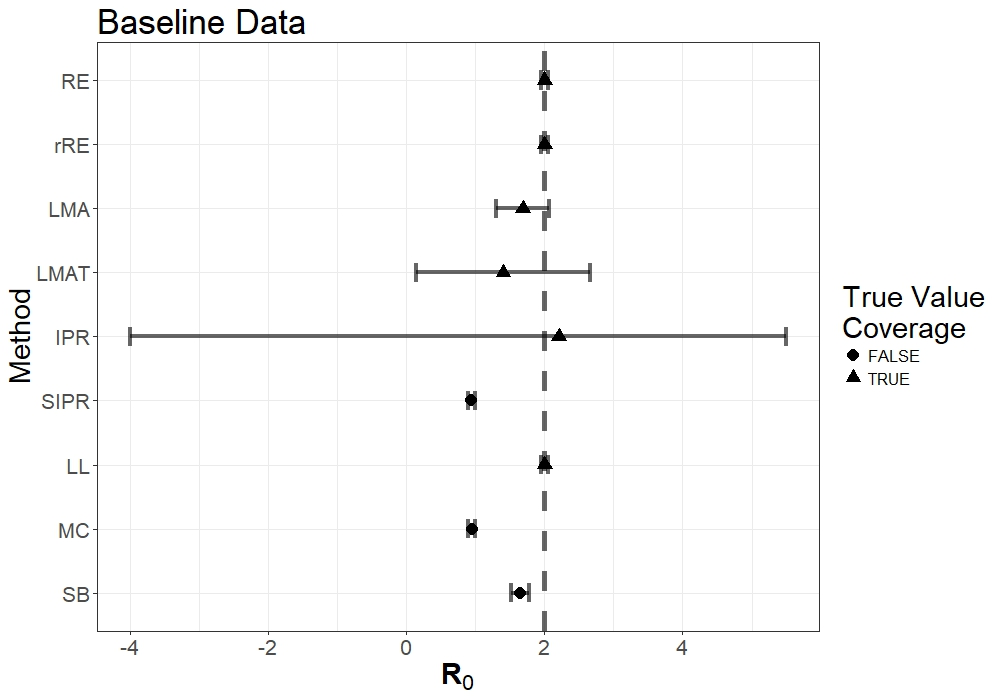
\includegraphics[scale=0.5]{images/BaseBase.jpeg}
  \caption{Forest plots of estimates of $\rr$ for the \xxsir methods for the baseline data set $(\beta=.06, \gamma=.03, O=365, X(0)=99950, Y(0)=50, Z(0)=0, \sigma_X=100, \sigma_Y=5, N=10^5)$.  The points are the estimates of $\rr$ and the lines denote $\pm 2\cdot $Std. Err.  The vertical, dashed line is the true $\rr$ value.}\label{fig:baseline-res}
  \end{figure}

\begin{table}[H]	
	\centering
	\begin{tabular}[t]{l|r|r}
		\hline
		Model & Estimate & Std. Err\\
		\hline
		RE & 1.9999711 & 0.0056\\
		\hline
		rRE & 1.9997340 & 0.0050\\
		\hline
		LMA & 1.6863640 & 0.1886\\
		\hline
		LMAT & 1.4063227 & 0.6309\\
		\hline
		IPR & 4.4203632 & 12.3593\\
		\hline
		SIPR & 1.8870824 & $<$ 1e-04 \\
		\hline
		LL & 1.9998072 & 0.0002\\
		\hline
		MC & 0.9485555 &  $<$ 1e-04 \\
		\hline
		SB & 1.6495023 & 0.0672\\
		\hline
	\end{tabular}
        \caption{Baseline Data $(\beta=.06, \gamma=.03, T=365, X(0)=99950, Y(0)=50, Z(0)=0, \sigma_X=100, \sigma_Y=5, N=10^5)$, $\rr$ Estimates and Standard Errors}\label{tab:baseline-res}
\end{table}

Overall, in Figure \ref{fig:baseline-res}, we see a wide variation in the estimates of and the standard errors for $\rr$ depending on the method used.  The methods of RE, rRE, LMA, LMAT, IPR, and LL all result in a CI that covers the true value of $\rr=2$.  Of these, LMAT and IPR result in a CI which contains 1, so we would not be able to say whether or the outbreak of a disease was due to random chance or not. On the other hand, many methods appear to underestimate the true $\rr$, and many of them have larger standard errors as well.  We would say that IPR's CI is uninformative. Additionally, MC and SIPR models seem to have unreasonably small standard errors.

From examining the full results in the Supplementary Material, the results of the baseline data set with normal error seem to be a good summary of the methods as a whole.  In Figure \ref{fig:baseline-res}, we see that the clear best methods to estimate $\rr$ are RE, rRE, and LL.  These three methods consistently outperform the other methods of accurately estimating $\rr$ with a reasonably small CI when varying a single parameter and holding the others as fixed from the generated data sets.

In particular, MC and SB almost never capture the true estimate and typically underestimate the true value of $\rr$.  This leads us to believe that these models are inadequate in capturing the effects of a disease following the SIR model.  Both models rely on parametric assumptions of simple underlying statistical distributions for the course of infection (binomial and Poisson, respectively) with time-invariant transmission parameters ($\alpha$ and $\lambda$).  These are good examples of why we need to consider other reasons for using a model other than the math resulting in a simple estimate.  That is not to say that variants of these models are unviable for modelling $\rr$, but they do not make for good defaults.  It is also an issue that these two methods consistently underestimate $\rr$, which could possibly lead to an unchecked epidemic.

IPR often produces reasonable point estimates for $\rr$ but simply has too large of a CI to be considered a useful estimate.  On the other hand, SIPR has a small CI that typically underestimates the true value of $\rr$.  Since SIPR smoothes the SIR curves, the peak of the infectious curve in particular is shrunken.  Since the peak value of number of infectious is crucial in estimating $\rr$ for SIPR, it makes sense that SIPR underestimates this result.  Additionally, LMA and LMAT are generally prone to underestimating $\rr$ and have large and generally uninformative CIs.

Of the three well-performing methods, RE and rRE seem to be slightly more robust to parameter variation than LL.  This is mostly due to the fact that LL produces such small CIs that even a small discrepancy in estimation of $\rr$ can cause the CI to not capture the true value of $\rr$.

However, we do see instances where LL completely outperforms RE and rRE such as in the case where the initial percent of infectious $\frac{I(0)}{N} \cdot 100\%$ is $< .01$\%. In Figure \ref{fig:ar-small-I}, we examine the data set generated with autoregressive monotonic error, our most stringent data structure, with varying levels of initial percent of infectious individuals.  When $\frac{I(0)}{N} \cdot 100\%$ $< .01$\%, RE and rRE tend to overestimate $\rr$ and have large CIs.  However, LL accurately estimates $\rr$ even when the initial percentage of infectious is very small.  This is also true for the other error sets (see the Supplementary Materials for more details).

\begin{figure}[H]
	\centering
	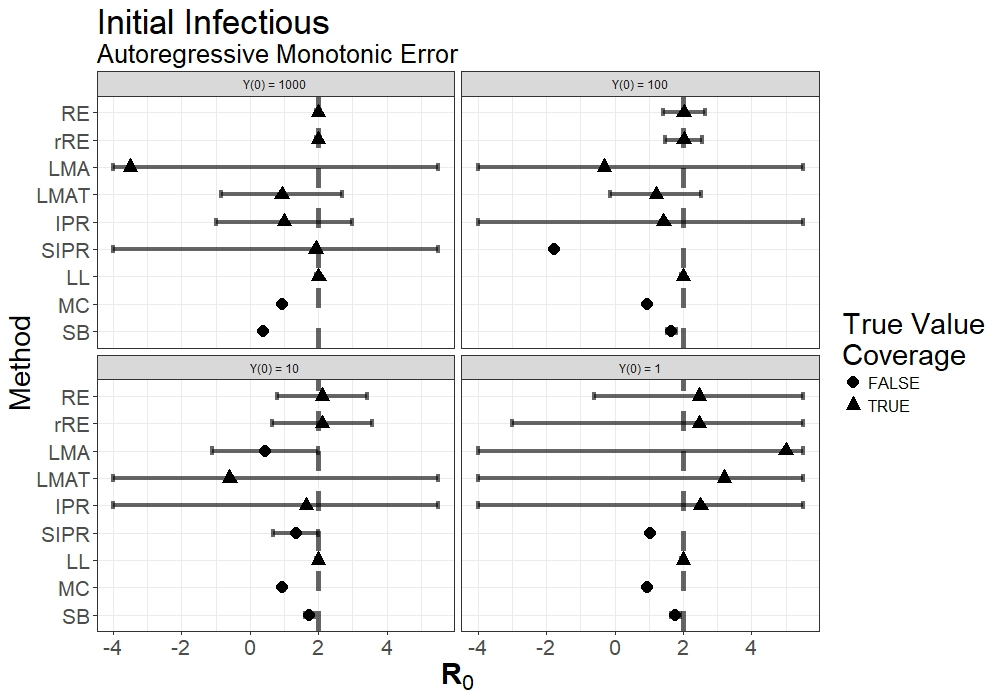
\includegraphics[scale=0.5]{images/start_arm.jpeg}
	\caption{Forest plots of estimates of $\rr$ for the \xxsir methods for the Inits1-4 data sets $(\beta=.06, \gamma=.03, T=365,  Z(0)=0, \sigma_X=100, \sigma_Y=5, N=10^5)$.  The points are the estimates of $\rr$ and the lines denote $\pm 2\cdot $Std. Err.  The vertical line is the true $\rr$ value.}\label{fig:ar-small-I}
\end{figure}

One interesting feature we see in the results is that RE and rRE can result in very different estimations and CIs, which may seem unintuitive since rRE is a simple reparametrization of RE.  For example, in Figure \ref{fig:ar-r0}, we see that when the true value of $\rr$ is 1, rRE has a much smaller CI than RE, which may be one reason to prefer rRE to RE.  This figure also helps to show that RE and rRE are robust to extreme values of $\beta$ and $\gamma$ and hence extreme values of $\rr$.

\begin{figure}[H]
	\centering
	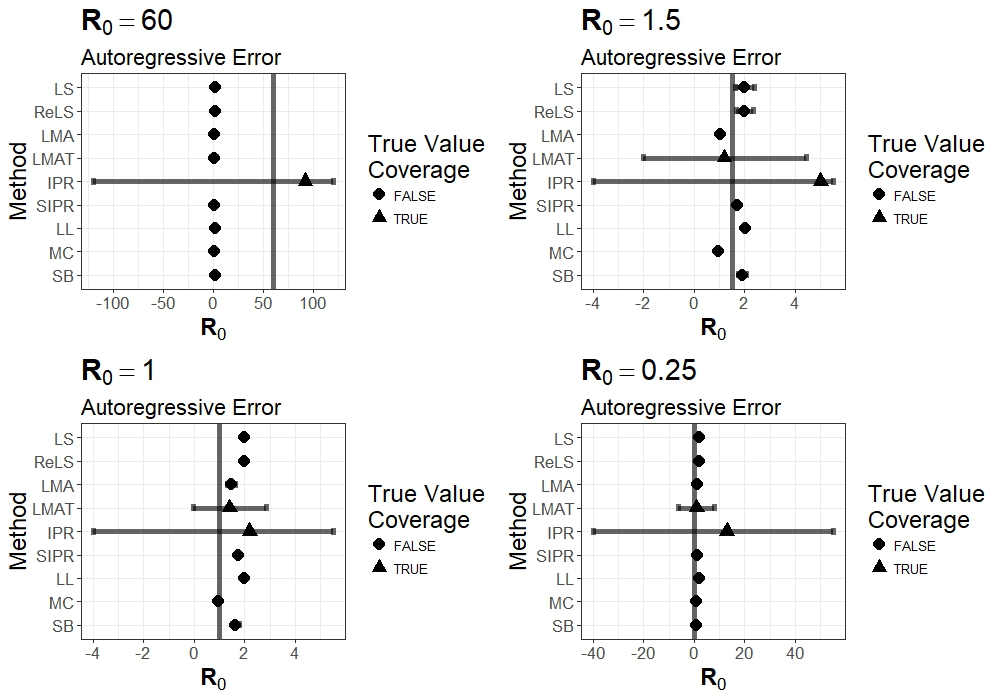
\includegraphics[scale=0.5]{images/parchange_ar.jpeg}
	\caption{Forest plots of estimates of $\rr$ for the \xxsir methods for the infrec1-4 data sets $(T=365, X(0)=99950, Y(0)=50, Z(0)=0, \sigma_X=100, \sigma_Y=5, N=10^5)$.  The points are the estimates of $\rr$ and the lines denote $\pm 2\cdot $Std. Err.  The vertical line is the true $\rr$ value.}\label{fig:ar-r0}
\end{figure}


%% robust to different error assumptions
 In Figure \ref{fig:err-rob} we plot the standardized residuals of $\rr$ focusing on the three best methods: RE, rRE, and LL.  Reassuringly, we find that $\hat{\rr}$ estimates from RE and rRE seem to be generally robust to the error structure.  ((What's up with varying $\rr$ values??))

\begin{figure}[H]
	\centering
	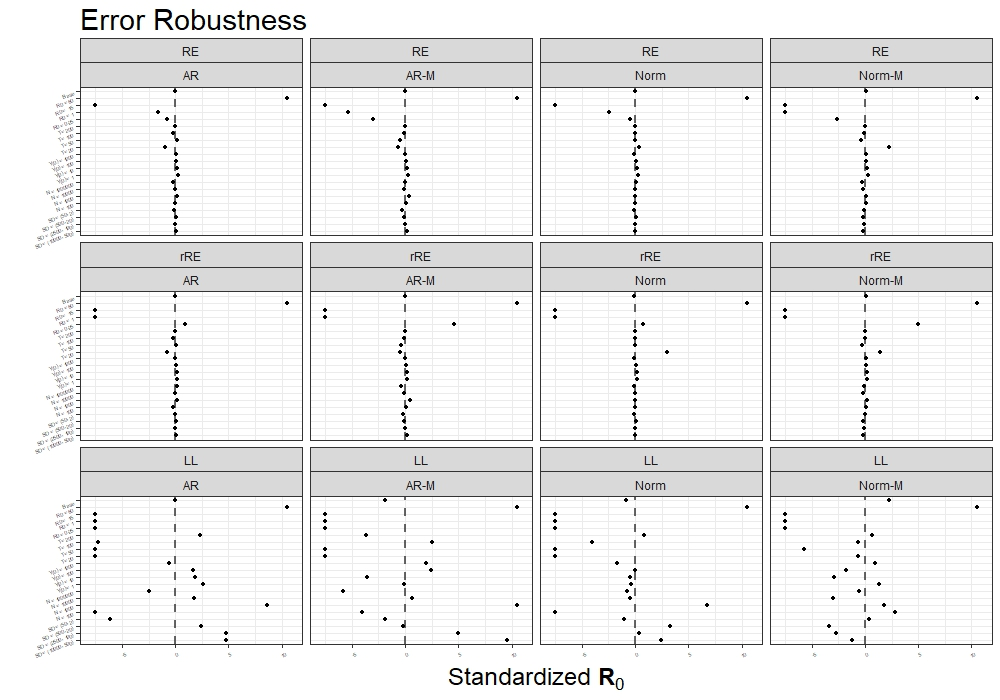
\includegraphics[scale=0.5]{images/err_robust.jpeg}
	\caption{Standardized residuals $\frac{\left ( \hat{\rr} - \rr\right ) }{SE \left [\hat{\rr}\right ]}$ for the estimation methods of RE, rRE, and LL faceted by the four error structures.  The dashed line is the true value of $\rr$.}\label{fig:err-rob}
\end{figure}

%% model misspecification is fairly robust
We also examine circumstances where the data is generated from underlying models different from the SIR model.  The results are plotted in Figure \ref{fig:mod-rob}  All three sets of data sets generated by the non-SIR models result in poor estimates of $\rr$, meaning that even our best estimation techniques fail under model misspecification.

\begin{figure}[H]
	\centering
	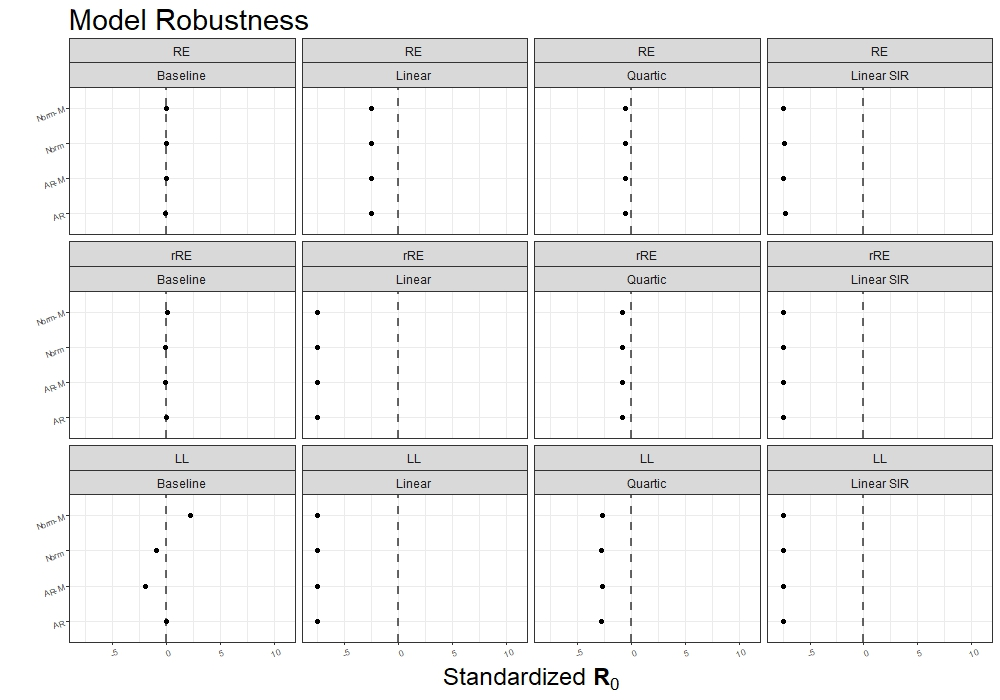
\includegraphics[scale=0.5]{images/model_robust.jpeg}
	\caption{Standardized residuals $\frac{\left ( \hat{\rr} - \rr\right ) }{SE \left [\hat{\rr}\right ]}$ for the estimation methods of RE, rRE, and LL faceted by the four model structures (SIR, Poly1, Poly4, and LSIR).  The dashed line is the true value of $\rr$.}\label{fig:mod-rob}
\end{figure}

%% small N or small  T can lead to bad results. Also large sig X, sig Y, and small gamma

Generally, we find that when $N$, the number of individuals decreases, then the CIs of our estimates generally increase.  This is evidence of the  central limit theorem (CLT) taking effect.   When the noise parameters $\sigma_X$ or $\sigma_Y$ increase then the CI lengths of our estimates also generally increase.  For both small $N$ and large $\sigma_X$ or $\sigma_Y$, we find that the point estimates of $\rr$ seem to be unbiased but may have large CIs depending on the other parameters.

We find the parameter $T$ to be particularly important, as shown in Figure \ref{fig:timediff}.  For one, it can play a role similar to that of $N$, directly giving the researcher more data for a larger $T$.  Thus, larger $T$ may result in smaller CIs due to the CLT.  However, $T$ also plays an even more important role than $N$ in estimating $\rr$.  We see in Figure \ref{fig:timediff}, for RE and rRE, about 50 time points are required to accurately capture the true estimate of $\rr$.  For LL, we see that at least 100 time points are required.

\begin{figure}[H]
	\centering
	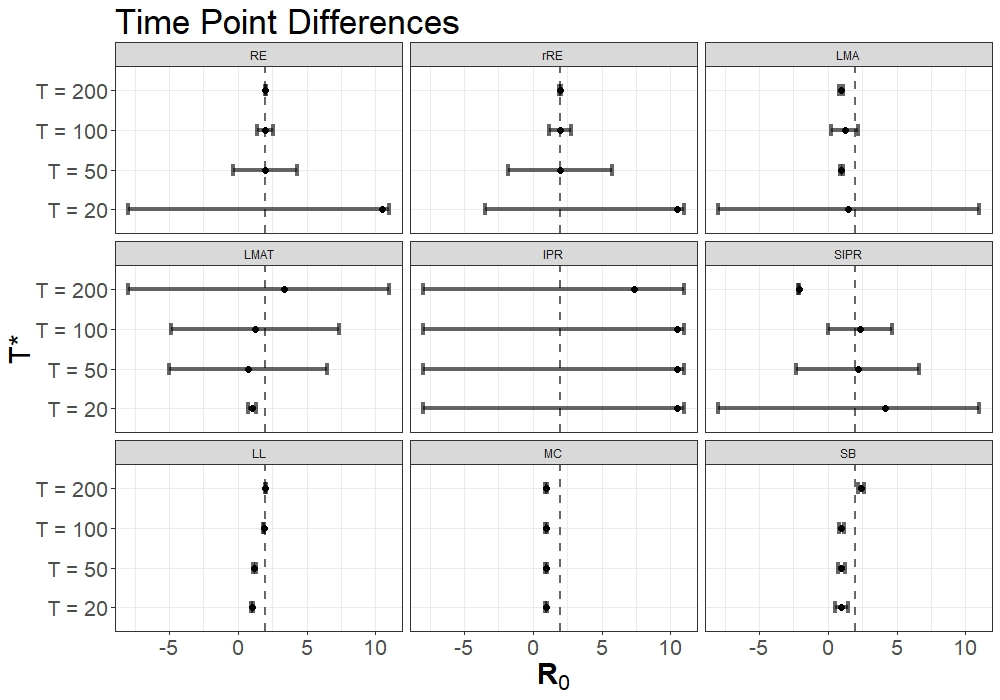
\includegraphics[scale=0.5]{images/timediff.jpeg}
	\caption{Forest plots of estimates of $\rr$ for the \xxsir methods for the baseline data sets with normall error structure $(\beta=.06, \gamma=.03, X(0) = 99950, Y(0)=50, \sigma_X=100, \sigma_Y=5, N=10^5)$.  The points are the estimates of $\rr$ and the lines denote $\pm 2\cdot $Std. Err.  The vertical line is the true $\rr$ value.}\label{fig:timediff}
      \end{figure}

      In the previous plots, we assume that we are collecting incidence and recovery date every day.  However, it is also possible to observe weekly, monthly, or even quarterly incidence and recovery data, for example.  In Figure \ref{fig:obs}, we explore estimates of $\rr$ using the data collected at different time periods for our baseline data structure with a full year's worth of data.  We find that we can reliably estimate $\hat{\rr}$ regardless of the collection period.  This is likely due to the previously discussed relationship between $\rr$ and the final size of the epidemic.  (ADD IN)

However, if we are given only 200 days worth of data, we find that the collection period size does result in different estimates.  PLOT      
      

\begin{figure}[H]
	\centering
	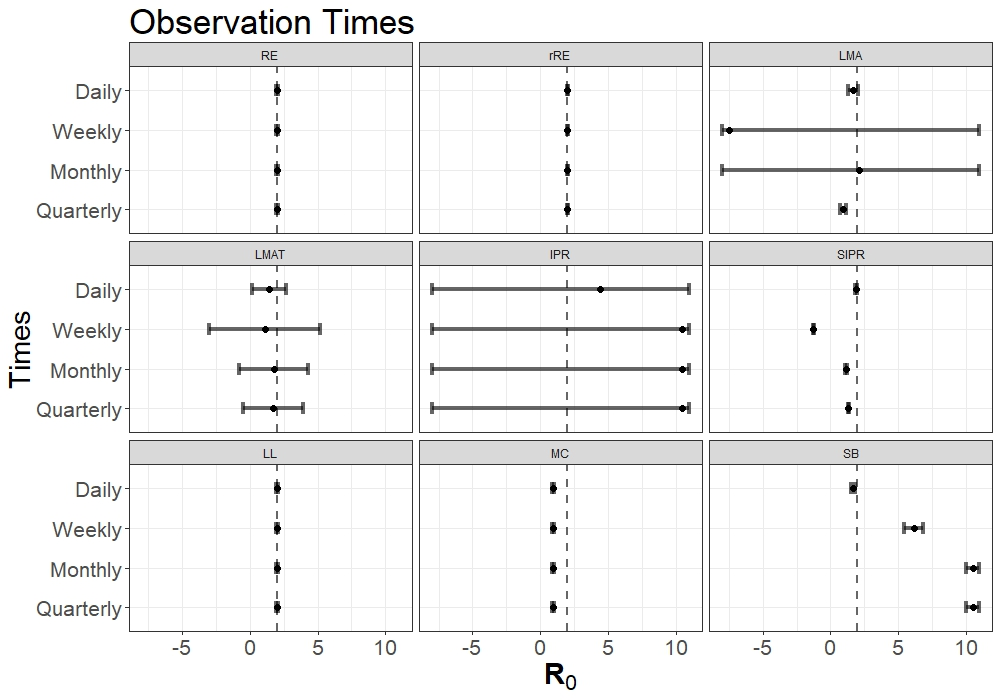
\includegraphics[scale=0.5]{images/obs.jpeg}
	\caption{Forest plots of estimates of $\rr$ for the \xxsir methods for the baseline data sets with normall error structure $(\beta=.06, \gamma=.03, X(0) = 99950, Y(0)=50, \sigma_X=100, \sigma_Y=5, N=10^5)$.  The points are the estimates of $\rr$ and the lines denote $\pm 2\cdot $Std. Err.  The vertical line is the true $\rr$ value.}\label{fig:obs}
\end{figure}

  





\subsection{Variance of $\rr$ estimation methods}\label{sec:sim-var-res}
We examine the variance methods used to estimate CIs for our estimates of $\rr$.  From the above results, we saw that methods such as RE, rRE, LL, and MC result in very small CIs.  On the other hand, methods such as IPR have consistently large CIs, to the point of being uninformative.  The other methods CI width seems to depend heavily on the initial parameters used.  Unsurprisingly, larger $\sigma_X$, $\sigma_Y$ values seem to correspond to larger CI sizes.  On the other hand, large $N$ and $T$ values seem to correspond to smaller CI sizes.   Having a larger percentage of initially infected individuals also seems to be associated with a larger CI.  We also see that having a very large $\rr$ value seems to have less effect on creating a large CI than does having a small value of $\rr$.  Perhaps surprisingly, the width of the CI seems to be independent of the error structure.

We estimate the variance through the delta method, posterior, and  block bootstrap and compare it to the empirical variance of $\rr$ for each of the methods, using 1000 data sets generated from the baseline data structure.

\subsubsection{Delta Method and Posterior}

Table \ref{tab:rep-samp} shows the mean and standard deviation of $\rr$ estimates produced by the models under 100 repetitions of the baseline conditions, with new noise generated each time. We want to compare the standard deviations of the estimates to the standard errors returned by each of the models for a single data set to asses how reliable those standard errors are. Overall, it appears than most of the models have standard error estimates that are larger than the actual standard deviation of the estimates under repeated sampling. In some cases, such as LL, LMA, and LMAT, the standard deviation and standard error estimates are fairly close. The least squares methods, RE and rRE, on the other hand, tend to overestimate the error by an order of magnitude. Finally, SIPR and SB, have individual standard error estimates that are smaller than the standard deviation of repeated estimates, meaning that they understate how much error is in the estimates.


\begin{table}[H]
	
	\centering
	\begin{tabular}[t]{l|r|r|r|r}
		\hline
		Model & Mean Estimate & Std. Dev. & Baseline Estimate & Baseline SE\\
		\hline
		RE & 2.0000 & 0.0003 & 1.9999 & 0.0058\\
		\hline
		rRE & 2.0000 & 0.0003 & 1.9997 & 0.0052\\
		\hline
		LMA & 1.8497 & 0.3339 & 1.9974 & 0.3900\\
		\hline
		LMAT & 1.4562 & 0.3577 & 1.3980 & 0.6028 \\
		\hline
		IPR & 4.5214 & 0.3705 & 2.5930 & 9.0408\\
		\hline
		SIPR & 1.7973 & 0.0951 & 0.9251 & $<$ 1e-04 \\
		\hline
		LL & 2.0000 & 0.0003 & 1.9998 & 0.0002\\
		\hline
		MC & 0.9486 & $<$ 1e-04 & 0.9486 & $<$ 1e-04\\
		\hline
		SB & 1.1330 & 0.4163 & 1.0000 & 0.0523\\
		\hline
	\end{tabular}
        \caption{Mean $\rr$ Estimates and Std. Devs, Delta Method/Posterior}
        \label{tab:rep-samp}
\end{table}

\subsubsection{Block Bootstrap}

Table \ref{tab:bb-samp} shows the mean and standard deviation of $\rr$ estimates produced by the models under 100 block bootstrap repetitions of the baseline data. The data were first detrended using the predictions of the compartment sizes at each time point from each of the models on the original data set. The block bootstrap algorithm was then applied on to the residuals from the predictions using a fixed block length. Only 5 of the models provide predictions of the size of the compartments and thus allow for detrending of the data. The ratio estimator and reparameterized model have a fairly accurate estimates of $\rr$ as well as very small standard errors. On the other hand, the linear approximation and smoothed IPR models both have very inaccurate estimates as well as very large standard errors of $\rr$.

\begin{table}[H]
	
	\centering
	\begin{tabular}[t]{l|r|r|r|r}
		\hline
		Model & Mean Estimate & Std. Dev. & Baseline Estimate & Baseline SE\\
		\hline
		RE & 1.9999 & 0.0003 & 1.9999 & 0.0058\\
		\hline
		rRE & 1.9998 & 0.0003 & 1.9997 & 0.0052\\
		\hline
		LMA & -0.9975 & 21.7161 & 1.9974 & 0.3900\\
		\hline
		LMAT & 1.5138 & 1.0485 & 1.3980 & 0.6028 \\
		\hline
		SIPR & 0.7762 & 2.6624 & 0.9252 & $<$ 1e-04 \\
		\hline
	\end{tabular}
	\caption{Mean $\rr$ Estimates and Std. Devs, Block Bootstrap}
	\label{tab:bb-samp}
\end{table}

Figure \ref{fig:coverage} shows the proportion of repetitions for both repeated sampling and block bootstrapping in which the 95\% confidence intervals of the estimates produced by the models covers the true $\rr$. The ratio estimator, reparameterized, and linear model approximation with all time points contain the true $\rr$ value in all of the confidence intervals. On the other hand, the smoothed IPR, Markov chain, and sequential Bayes models never cover the true $\rr$ in any of the confidence intervals.

\begin{figure}[H]
	\begin{center}
		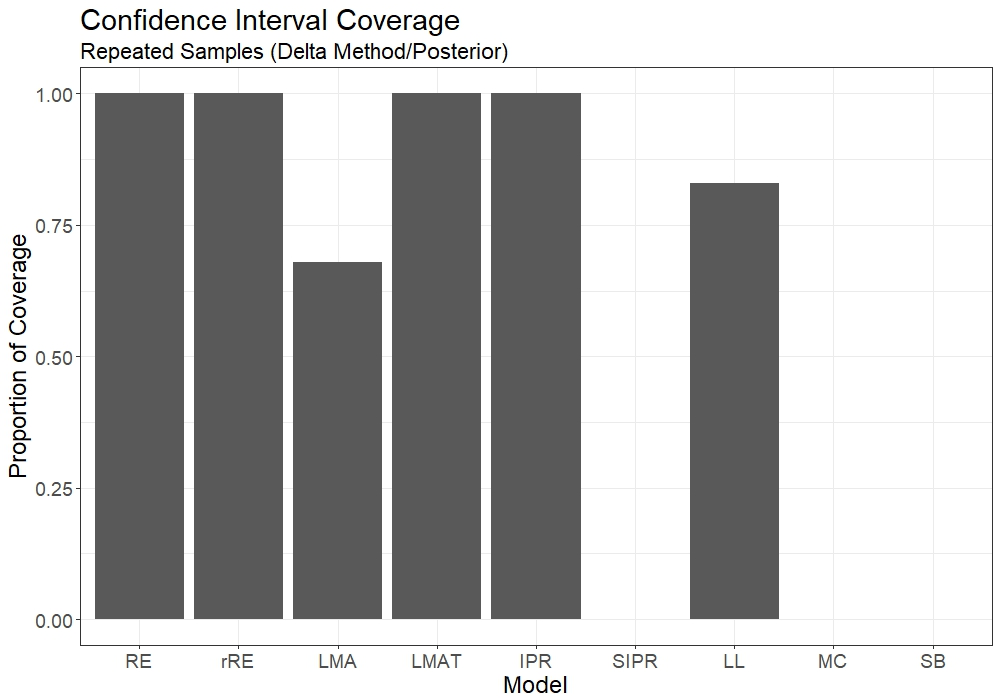
\includegraphics[scale=0.5]{images/coverage2.jpeg}
		\caption{Proportion of coverage of true $\rr$ of confidence intervals produced by repeated sampling for the applicable method (delta method or posterior).}
		\label{fig:coverage}	
	\end{center}
\end{figure}

\begin{figure}[H]
	\begin{center}
		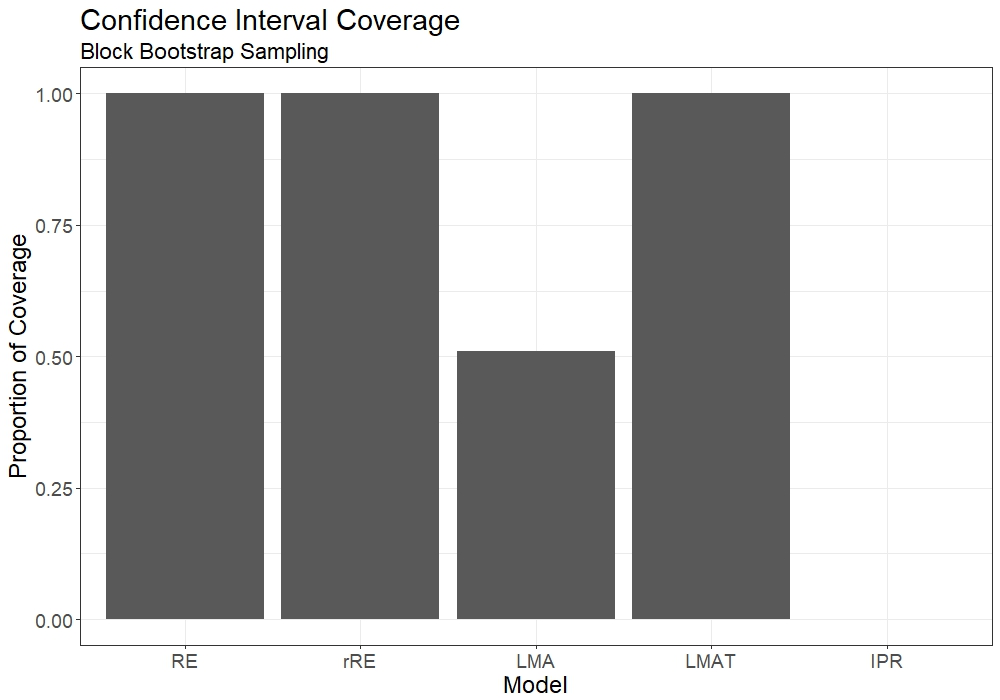
\includegraphics[scale=0.5]{images/coverage.jpeg}
		\caption{Proportion of coverage of true $\rr$ of confidence intervals produced by repeated sampling for block bootstrapping.}
		\label{fig:coverage}	
	\end{center}
\end{figure}



      \subsection{Application to USA H1N1 data}\label{sec:real-data}
      We apply our methods using data from the 2009 H1N1 pandemic in the United States.

      \subsubsection{USA H1N1 Influenza A 2009 data}
      The data is from the Center of Disease Control and Prevention's (CDC) FluView \citep{cdc-fluview}.  The data source is ILINet and is the national level data.  We use the same date range as in \cite{towers2009}, namely Epiweeks 21-33 (May 23, 2009-August 22, 2009).  From the United States Census Bureau, we use the population estimate of the USA as of April 1, 2010 of $N=308,740,000$ individuals \citep{census-2010}.  The main features in this data set are weighted influenza like illness (wILI) for a given week (Epiweek).  The wILI values are estimated based on the number of patients diagnosed with influenza like illness and weighted based on the reporting locations.  To obtain weekly incidence from wILI, we use $J(t) = \textnormal{wILI}(t) / 100 \cdot N$.  Then to obtain prevalence $I(t)$, we use the relation of $I(t) = \gamma^{-1}J(t)$, where $\gamma$ is the inverse of the expected time to recovery, which we here use as $\gamma^{-1} = \frac{3}{7}=.429$ weeks \citep{vespignani2007}.  Then $S(t) = N - \sum_{s=0}^{t}J(s)$, the total population size minus the cumulative sum of the incidence, and $R(t) = N - S(t) - I(t)$.  As prior knowledge of $\gamma$ is used to estimate our data for $I$, we expect it to influence our estimates of $\rr$.  The data is summarized in Table \ref{tab:h1n1-data}.


% Please add the following required packages to your document preamble:
% \usepackage{booktabs}
\begin{table}[H]
\centering
\begin{tabular}{@{}ll@{}}
\toprule
Feature       & Notes                                                                   \\ \midrule
Disease       & H1N1 Pandemic Influenza A                                                 \\ 
Source        & CDC FluView (\url{https://www.cdc.gov/flu/weekly/})      \\
Year          & 2009                                                                    \\
Date(s)          & May 23-August 22 (Epiweeks 21-33)                                       \\
Location      & USA                                                                     \\
Population    & $N$=308,740,000 people                                                  \\
  Avg. Duration $\left ( \gamma^{-1}\right )$ & $\frac{3}{7}$ weeks\\
  Raw data & Weekly wILI reports\\
  Final data & S$(t)$, I$(t)$, R$(t)$ \\\bottomrule
\end{tabular}
\caption{Summary of the data used to estimate $\rr$ during the 2009 H1N1 influenza pandemic in the USA.  We follow the data collection procedure described in \cite{towers2009}.}
\label{tab:h1n1-data}
\end{table}

\begin{figure}[H]
  \centering
  \includegraphics[width=\textwidth]{images/h1n1-sir.pdf}
  \caption{Data from H1N1 influenza 2009 in the USA.  Weekly wILI is reported, which we transform into S, I, and R counts shown for weeks (start of weeks: April 16-Aug. 27)  using $\gamma^{-1} = 3/7$ weeks.  The observations between the dotted lines denote the points used to estimate $\hat{\rr}$ in \cite{towers2009}.}
  \end{figure}
      

      \subsubsection{Results of H1N1 data}
      The results are shown below.  \cite{towers2009} report an estimate of $\hat{\rr} \in [1.50, 1.70]$.

\begin{figure}[H]
	\centering
	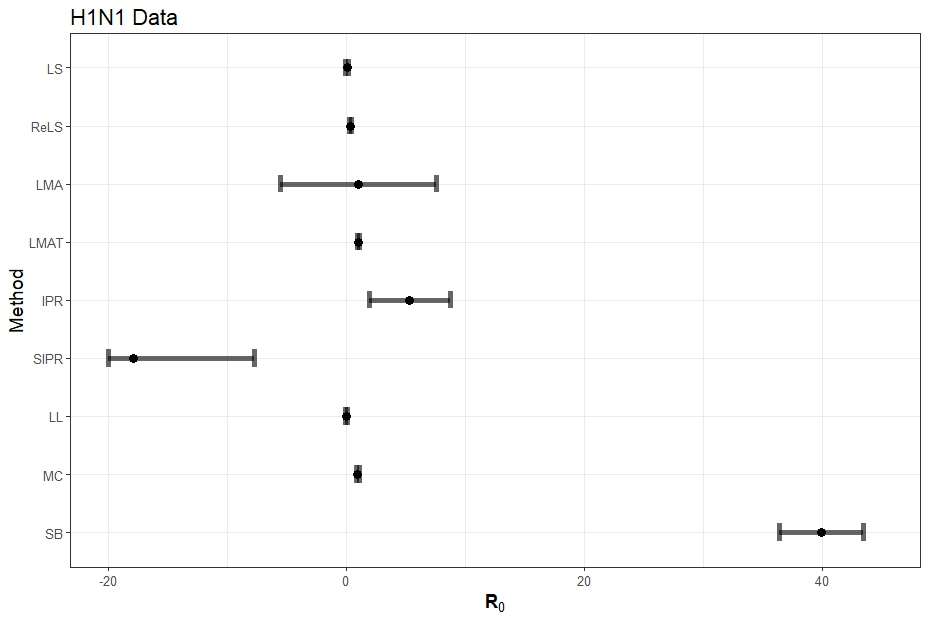
\includegraphics[width=\textwidth]{images/h1n1.jpeg}
	\caption{Results from SIR models on H1N1 data.}
\end{figure}

\begin{table}[H]
	
	
	\centering
	\begin{tabular}{l|r|r}
		\hline
		Model & Estimate & Std. Dev\\
		\hline
		RE & 1.1851 & 0.3540\\
		\hline
		rRE & 1.1851 & 0.0212\\
		\hline
		LMA & 4.3811 & 7.4772\\
		\hline
		LMAT & 1.2169 & 0.7584\\
		\hline
		IPR & 82.8540 & 24.5098\\
		\hline
		SIPR & 75.1963 & 16.2124\\
		\hline
		LL & 1.2128 & 0.0170\\
		\hline
		MC & 0.9486 & $<$ 1e-04 \\
		\hline
		SB & 2.0596 & 0.3292\\
		\hline
	\end{tabular}
	\caption{H1N1 Data, $\rr$ Estimates and Standard Errors}
\end{table}


      
\section{Discussion}\label{sec:discussion}

%% say what we said
%% say it
%% say it again


%% what is r0 and why it is important
In this paper, we examine $\rr$, the average number of secondary infections a primary individual generates when introduced into a completely susceptible population, in the context of the SIR model.  The quantity $\rr$ summarizes an epidemic into a single estimate in the hopes that infectious disease outbreaks may be compared to one another.  A value of $\rr > 1$ indicates an outbreak of a disease whereas a value of $\rr < 1$ indicates that no outbreak will occur.  Thus, it is critical to not only estimate the value of $\rr$ but also a corresponding CI.  Overestimating $\rr > 1$ during an ongoing epidemic may result in a waste of resources in prevention and control measures; underestimating $\rr < 1$ may result in a worldwide crisis.

In Table \ref{tab:r0-real-ex}, we provide estimates for $\rr$ that have appeared over the past three decades for HIV, Zika, Ebola, influenza, H1N1 influenza, and measles in different locations throughout the world.  Each of these estimates is greater than $1$, which makes sense as we tend to care more when a disease has the potential outbreak.  The largest $\rr$ point estimate we have seen is for measles at $\rr=17$ in England in the 20th century, and the smallest is $\rr=1.08$ for HIV in Portugal in the 21st century.
%% r0 as a property of the model
The quantity $\rr$ may summarize an epidemic, accounting for temperature, seasonality, location, and genetics of a disease, but it is still a property of the model.  Namely, how individuals progress through an epidemic (e.g. susceptible to infectious to recovered compartments) influences how we view $\rr$.  We thus should compare estimates for $\rr$ for a fixed epidemic model.  Here, we limit our analysis to estimates of $\rr$ derived from the SIR model.  Then $\rr = \frac{\beta}{\gamma}$ where $\beta$ is the rate of infection and $\gamma$ is the rate of recovery.  As a consequence, we need to estimate $\rr$ from not only the number of infections but also the number of individuals recovering at each time step.


%% the methods we chose and why we chose them
Additionally, the SIR model assumes monotoncity of S and R compartments which can make estimating $\rr$ more difficult, especially in terms of the CIs since the usual assumption of Gaussian noise may be violated due to the non-symmetric nature of the noise.  We examine \wxxsir methods to estimate $\rr$ which include least squares optimization, polynomial approximations, estimates from incidence and variance, a log-linear model, a Markov chain method, and a simple Bayesian method.  Although, this is not an exhaustive list of methods used to estimate $\rr$ from the SIR model, we believe it covers common and popular methods used throughout the decades.  We overview the details of methods in Section \ref{sec:methods}.

%% the importance of variance and testing
Each of the \wxxsir methods results in an estimate of $\rr$, $\hat{\rr}$.  We also estimate a 95\% CI for the  $\rr$ estimate.  Although, many researchers report intervals via sensitivity analysis (how the estimate changes with small variations in the underlying parameters), the ranges of these parameters often do not incorporate any distributional assumptions about these estimated ranges and hence do not correspond to 95\% CIs.  We provide three statistical methods to estimate the standard error of $\hat{\rr}$ and use the interval $\left [\hat{\rr} \pm 2\hat{SE}\left (\hat{\rr} \right ) \right ]$ as our 95\% CI.  We hope that these intervals will provide guidance on how to create more meaningful intervals when estimating $\rr$ and discerning which diseases are more severe than others, and whether the true $\rr >1$.

We compare the the estimates of $\rr$ for the \wxxsir methods using a series of simulations.  We generate different simulated data sets under different noise assumptions and estimate $\rr$ using each of these data sets.  We then analyze estimates of $\rr$ while varying individual parameters of the model including the infection and recovery parameters, the total amount of data, the initial percent of infectious and susceptible individuals, the standard deviation of the noise used to generate the simulated data, and the total number of individuals in a population.  We also analyze the model under misspecification, that is when a model other than the SIR model is used to generate the simulated data sets.  Finally, we compare our variance methods to one another and analyze the coverage of our methods.

%%%%%%%%%%%%%%%%%%%%%%%%%%%%%%%%%%%%%%%%%%%%%%%%%
%%RESULTS
%%%%%%%%%%%%%%%%%

Overall, we recommend based on our analysis:
\begin{itemize}
  \item RE and rRE provide the most accurate estimates of $\rr$
  \item LL results in close point estimates but occasionally has too small standard errors
  \item The specific MC and SB methods presented here do not seem to fit our generated data well
  \item There is not much difference in estimations of $\rr$ due to different error generating processes
  \item Very small values of $\gamma$ can result in very poor estimates of $\rr$
  \item 100 data points seems to be a reasonable number of data points to have enough power for testing that $\rr > 1$ and 50 seems to be too few
  \item The larger the number of initially infectious individuals is, the smaller the CIs for $\rr$ are
  \item The noisier the epidemic data is, the larger our CIs for $\rr$ are
  \item Estimations of $\rr$ are fairly robust to the misspecified data sets we presented, at least for the methods of RE, rRE, and LL
  \item Block bootstrap matches the empirical variance through repeated sampling.
  \end{itemize}

$\rr$ is a difficult quantity to estimate, but we hope that our methods of estimation and simulations provide some guidance for researchers on how to generate statistically reliable estimates for $\rr$ and its CIs.  Our analysis is limited in scope to the SIR model, and in the future we would like to see how methods of estimating $\rr$ compare for models such as the SEIR and beyond.

%% results of simulations:
%% - data
%% - what parameters make a difference
%% - what methods perform best when
%% - misspecification
%% variance
%% beyond the sir model





The SIR estimation methods generally give reliable estimates when the data are from an underlying SIR model with little or no noise. However, the estimates from the various methods are generally much worse when the magnitude of the noise is larger, when the parameters of the model are unusual, and when the model is misspecified. We also see a large difference between the $\rr$ estimates and standard errors on the exact same data sets as well, even though all derived from the same model. Thus, when estimating $\rr$ based on an SIR or any other kind of compartment model, we need to take careful consideration.


\pagebreak

\bibliographystyle{apa}%Choose a bibliograhpic style
\bibliography{Master}


\appendix



\end{document}


%%%%%%%%%%%%%%%%%%%%%%
\textbf{Title:} 

\textbf{Author:} 

\textbf{Citation:} 

\textbf{Major themes:} 

\textbf{Notes:}
\\
%%%%%%%%%%%%%%%%%%%%%%




\begin{figure}[h]
\begin{center}
\includegraphics[width=4in]{images/mvhw7_3c.pdf}
\end{center}
\caption{
Biplots of the different continuous variables and their correlations.}\label{fig3c}
\end{figure}

%% two pictures whoa

\begin{figure}[h]
\centering


\begin{figure}[h]
\centering

\begin{subfigure}{.5\textwidth}
  \centering
  \includegraphics[width=1\linewidth]{images/mt_eda_cont_hists.pdf}
  \caption{Histograms of Arrival Delay and continuous covariates.  Arrival delay seems to have a right skewed distribution.  This may indicate that we will be transforming this variable later on.  After transforming Air Time and Distance by a log transformation, we don't really seem to have many outliers in our covariates.  We seem to have outliers in the CRS Dep. Time and Arrival Time; however, time is cyclical and so these are not, in fact outliers.}
  \label{hists}
\end{subfigure}%
\begin{subfigure}{.5\textwidth}
  \centering
  \includegraphics[width=1\linewidth]{images/mt_eda_cont_hists.pdf}
  \caption{\textcolor{red}{Placeholder}}
  \label{tabs1}
\end{subfigure}
\caption{}
\end{figure}


\begin{table}
\begin{tabular}{l | a | b | a | b}
\hline
\rowcolor{LightCyan}
\mc{1}{}  & \mc{1}{x} & \mc{1}{y} & \mc{1}{w} & \mc{1}{z} \    \hline
variable 1 & a & b & c & d \    variable 2 & a & b & c & d \\ \hline
\end{tabular}
\end{table}






%%
\begin{figure}
\centering
\begin{subfigure}{.5\textwidth}
  \centering
  \includegraphics[width=1\linewidth]{images/resids_full.pdf}
  \caption{}
  \label{residsf}
\end{subfigure}%
\begin{subfigure}{.5\textwidth}
  \centering
  \includegraphics[width=1\linewidth]{images/diags_full.pdf}
  \caption{ }
  \label{diagsf}
\end{subfigure}
\caption{}
\end{figure}




